\documentclass{article}
\usepackage[utf8]{inputenc}
\usepackage{graphicx}
\setlength{\parindent}{0pt}
\setlength{\parskip}{1em}

\title{FOAR705 - Learning Journal Week 6 - Software Carpentry Exercises}
\author{Jan Jugueta - 44828020}
\date{Week 6: 30/8/19 - 6/9/19}

\begin{document}

\maketitle

\section*{30/8/19 - 2:17pm}

Going through some Software Carpentry exercises in the FOAR705 class. Some useful commands:

\begin{verbatim}
    Ctrl + C 
\end{verbatim}
which is cancel.

\begin{verbatim}
    Ctrl + D
\end{verbatim}
which is disconnect.

\section*{30/8/19 - 2:37pm}

Still practicing some Shell things. Practicing how to navigate again.

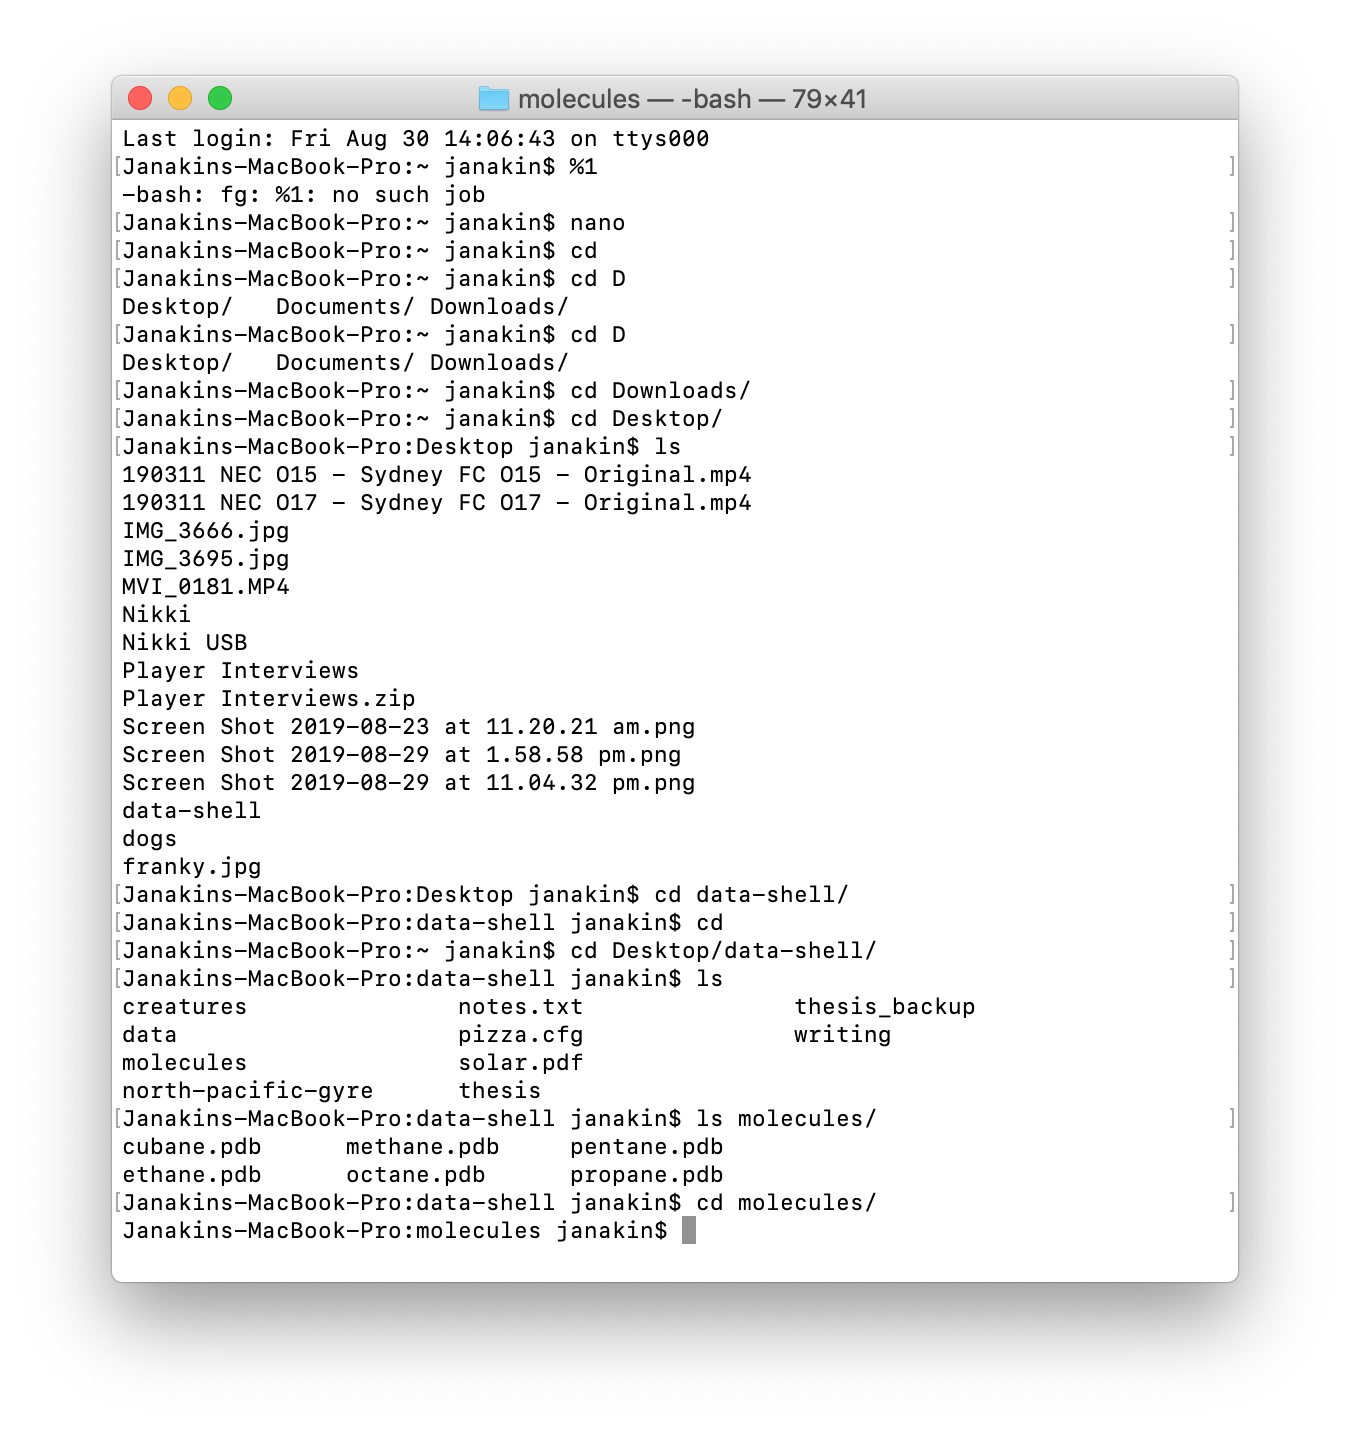
\includegraphics[width=\textwidth]{figa.png}

\section*{30/8/19 - 2:43pm}

The command \begin{verbatim}
    history
\end{verbatim}
shows all the commands you have used previously.

The command \begin{verbatim}
    >
\end{verbatim}
redirects.

The command \begin{verbatim}
    cat
\end{verbatim}
opens files.

\section*{30/8/19 - 2:58pm}

My first pipe attempt.

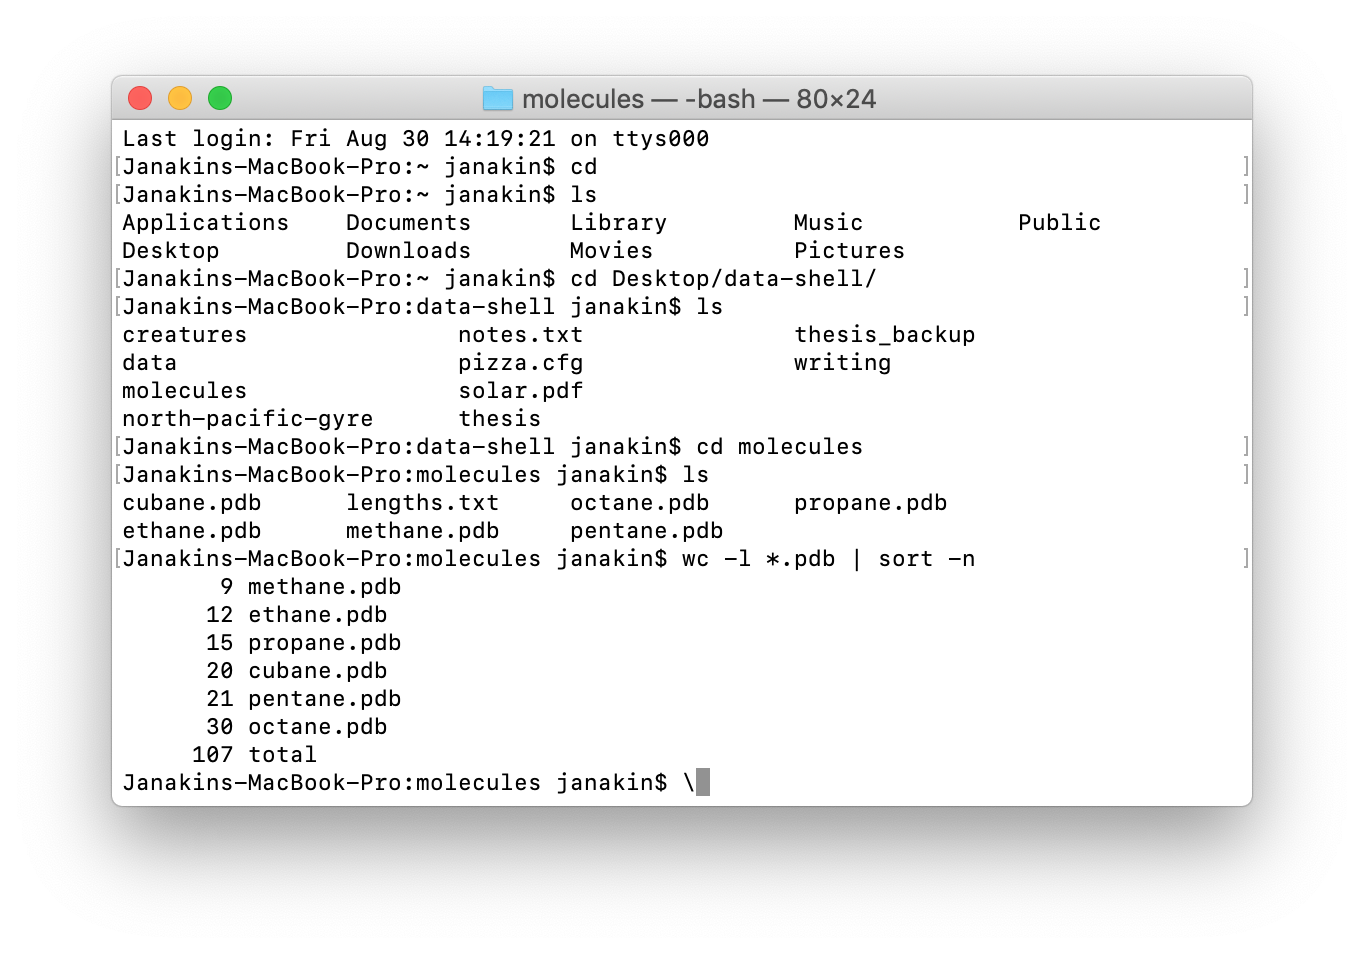
\includegraphics[width=\textwidth]{figb.png}

\section*{4/9/19 - 12:38pm}

Now time to do the SW Carpentry exercises properly. Continuing with Episode 4 \textbf{Pipes and Filters}

Have followed the instructions so far and no errors.

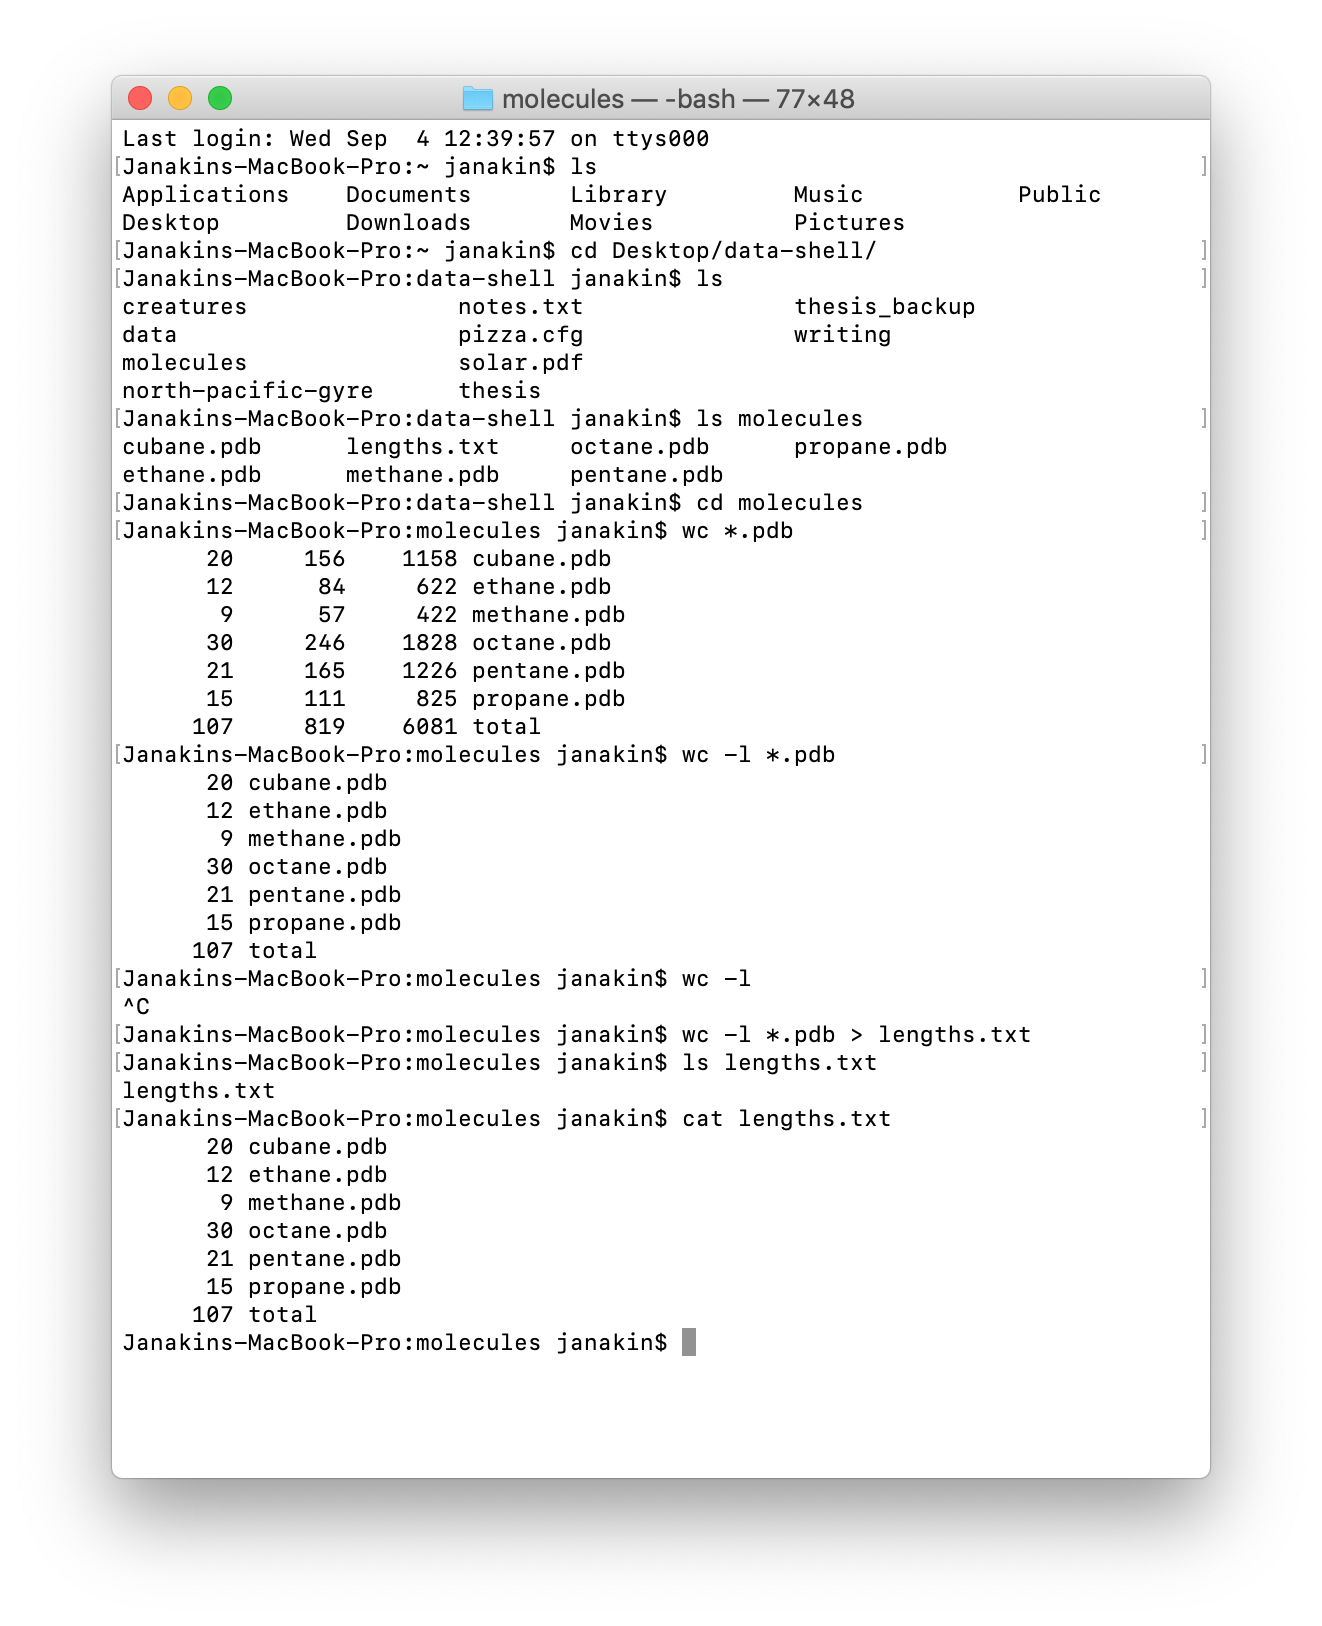
\includegraphics[width=\textwidth]{figc.png}

\section*{4/9/19 - 12:46pm}

The \begin{verbatim}
    less
\end{verbatim}
command in action.

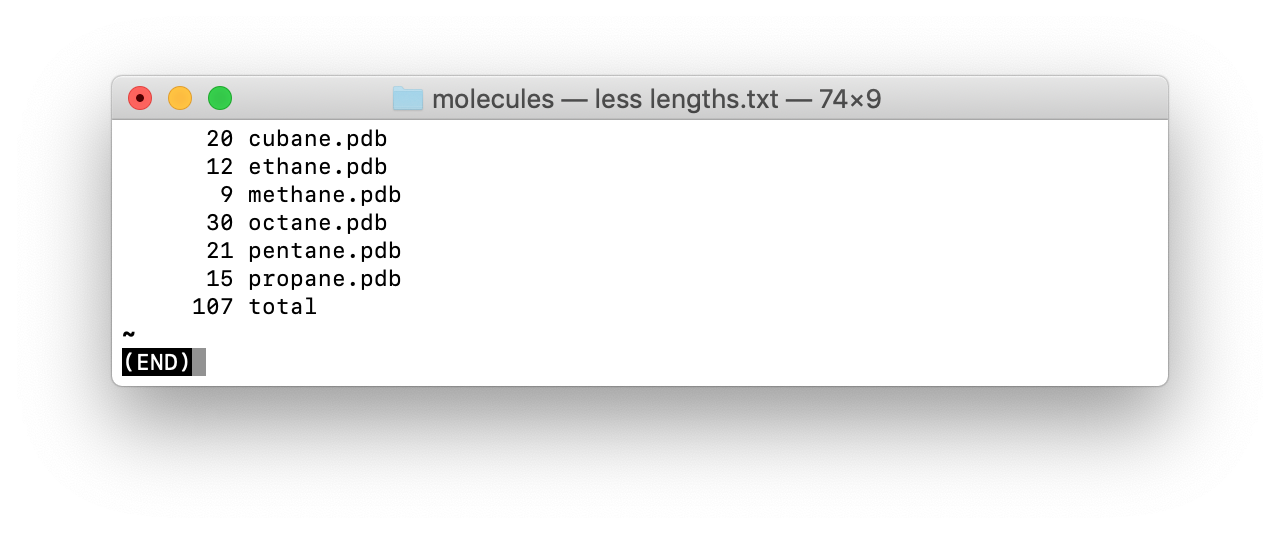
\includegraphics[width=\textwidth]{figd.png}

\section*{4/9/19 - 12:49pm}

The answer to the exercise \textit{What does sort -n Do?} is that \begin{verbatim}
    sort -n
\end{verbatim}
sorts purely numerically, not alphanumerically.

\section*{4/9/19 - 12:54pm}

Continuing on with the Episode. The following screenshots show the \begin{verbatim}
    sort -n lengths.txt > sorted-lengths.txt
    head -n 1 sorted-lengths.txt
\end{verbatim}
commands.

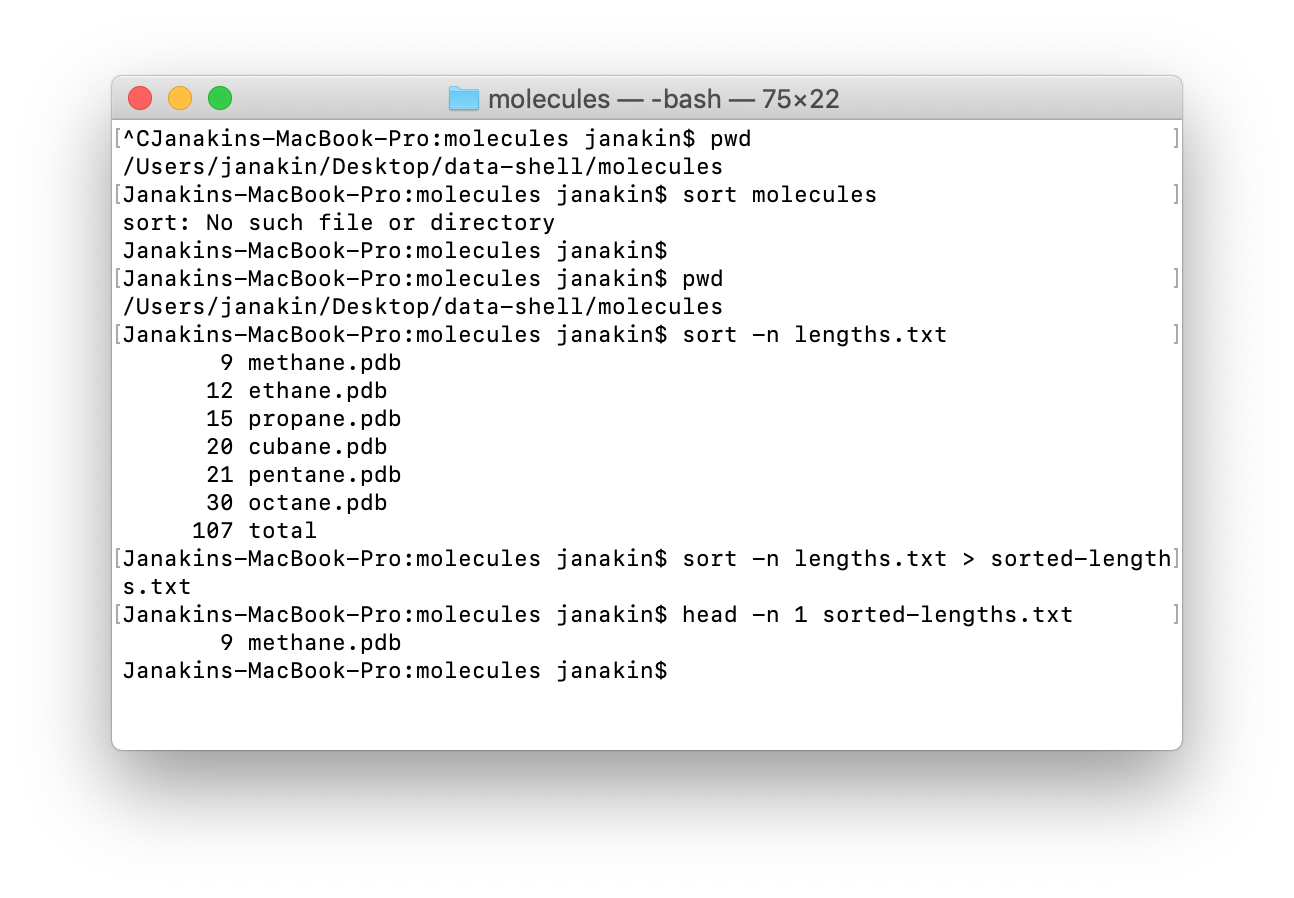
\includegraphics[width=\textwidth]{fige.png}

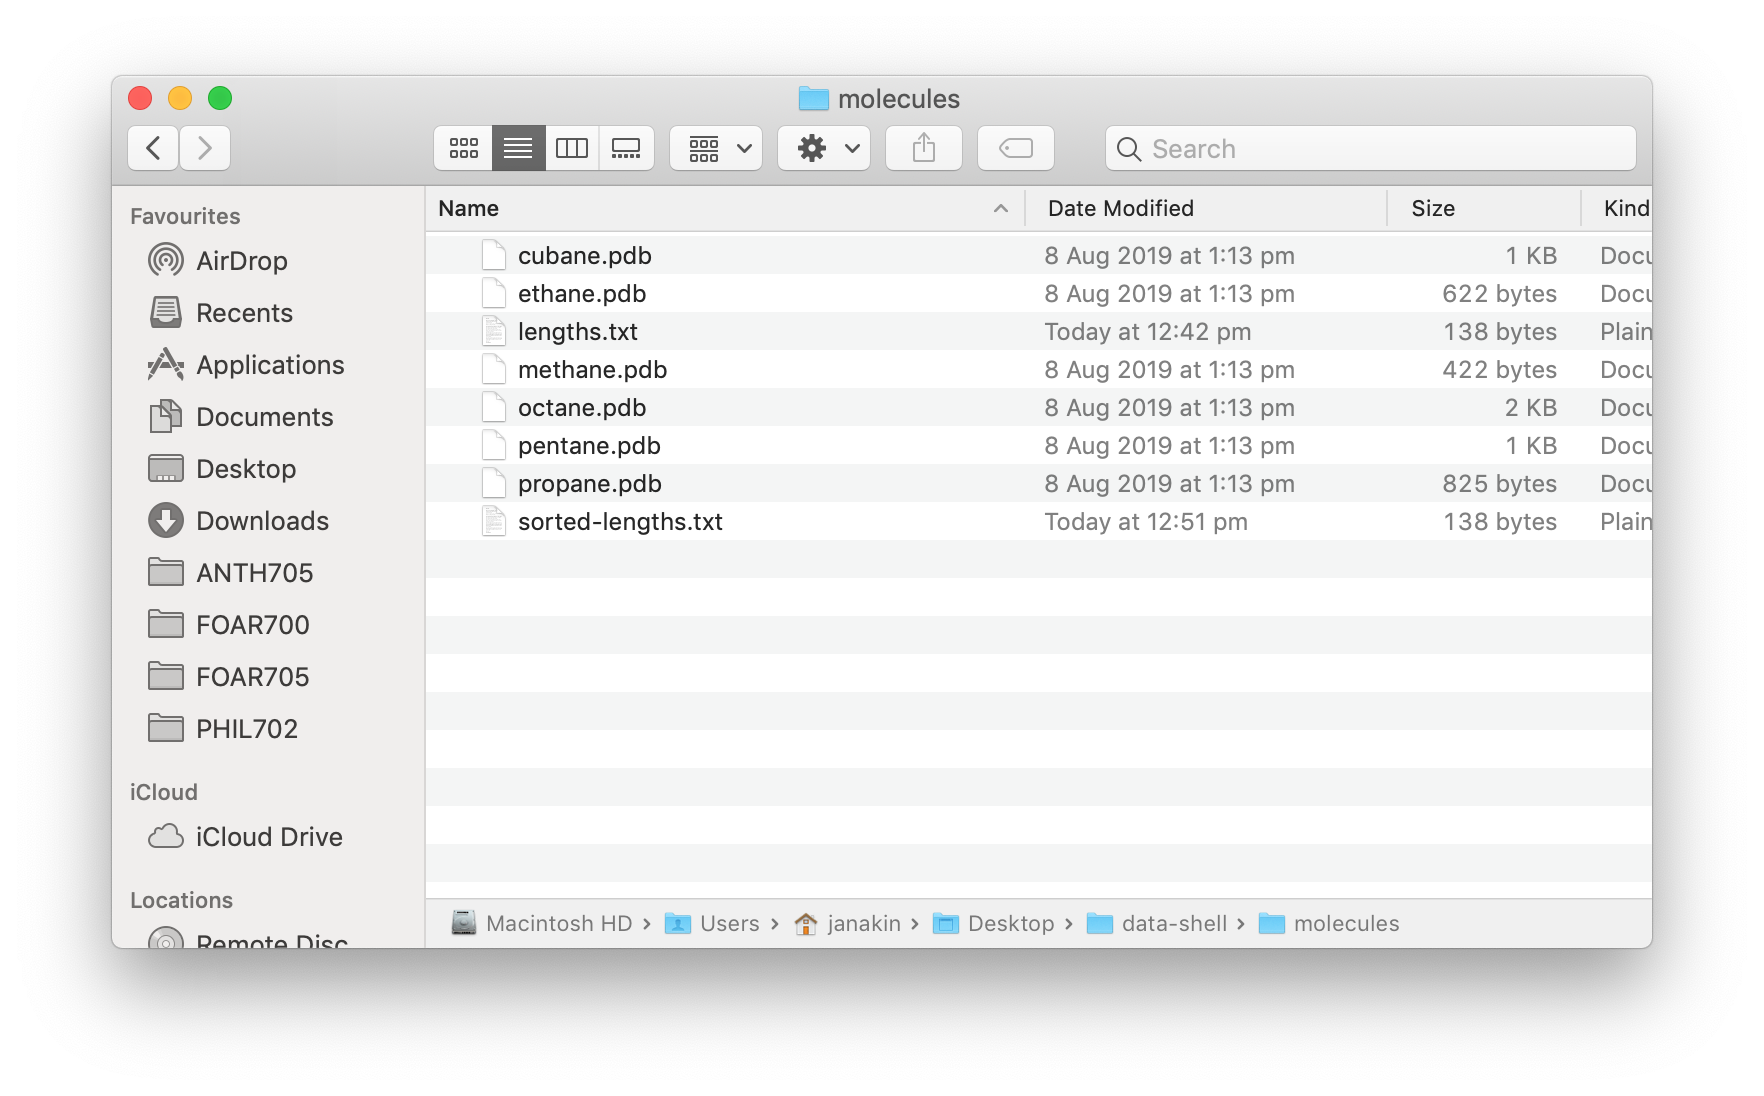
\includegraphics[width=\textwidth]{figf.png}

\section*{4/9/19 - 12:58pm}

What does \begin{verbatim}
    >>
\end{verbatim} mean?

Well, I've done exactly as the lesson says. But I still don't get it.

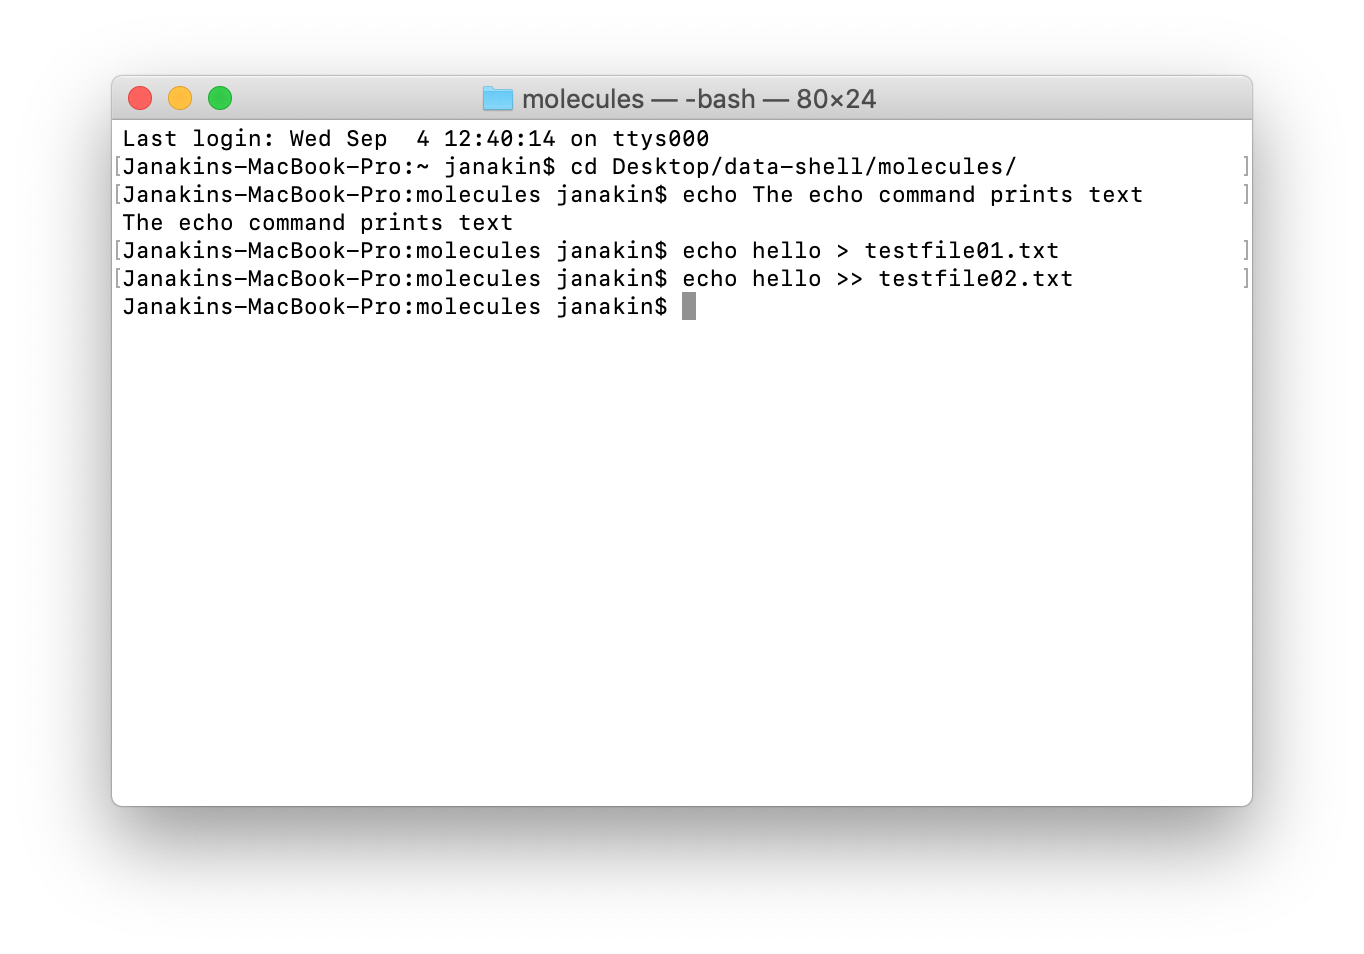
\includegraphics[width=\textwidth]{figg.png}

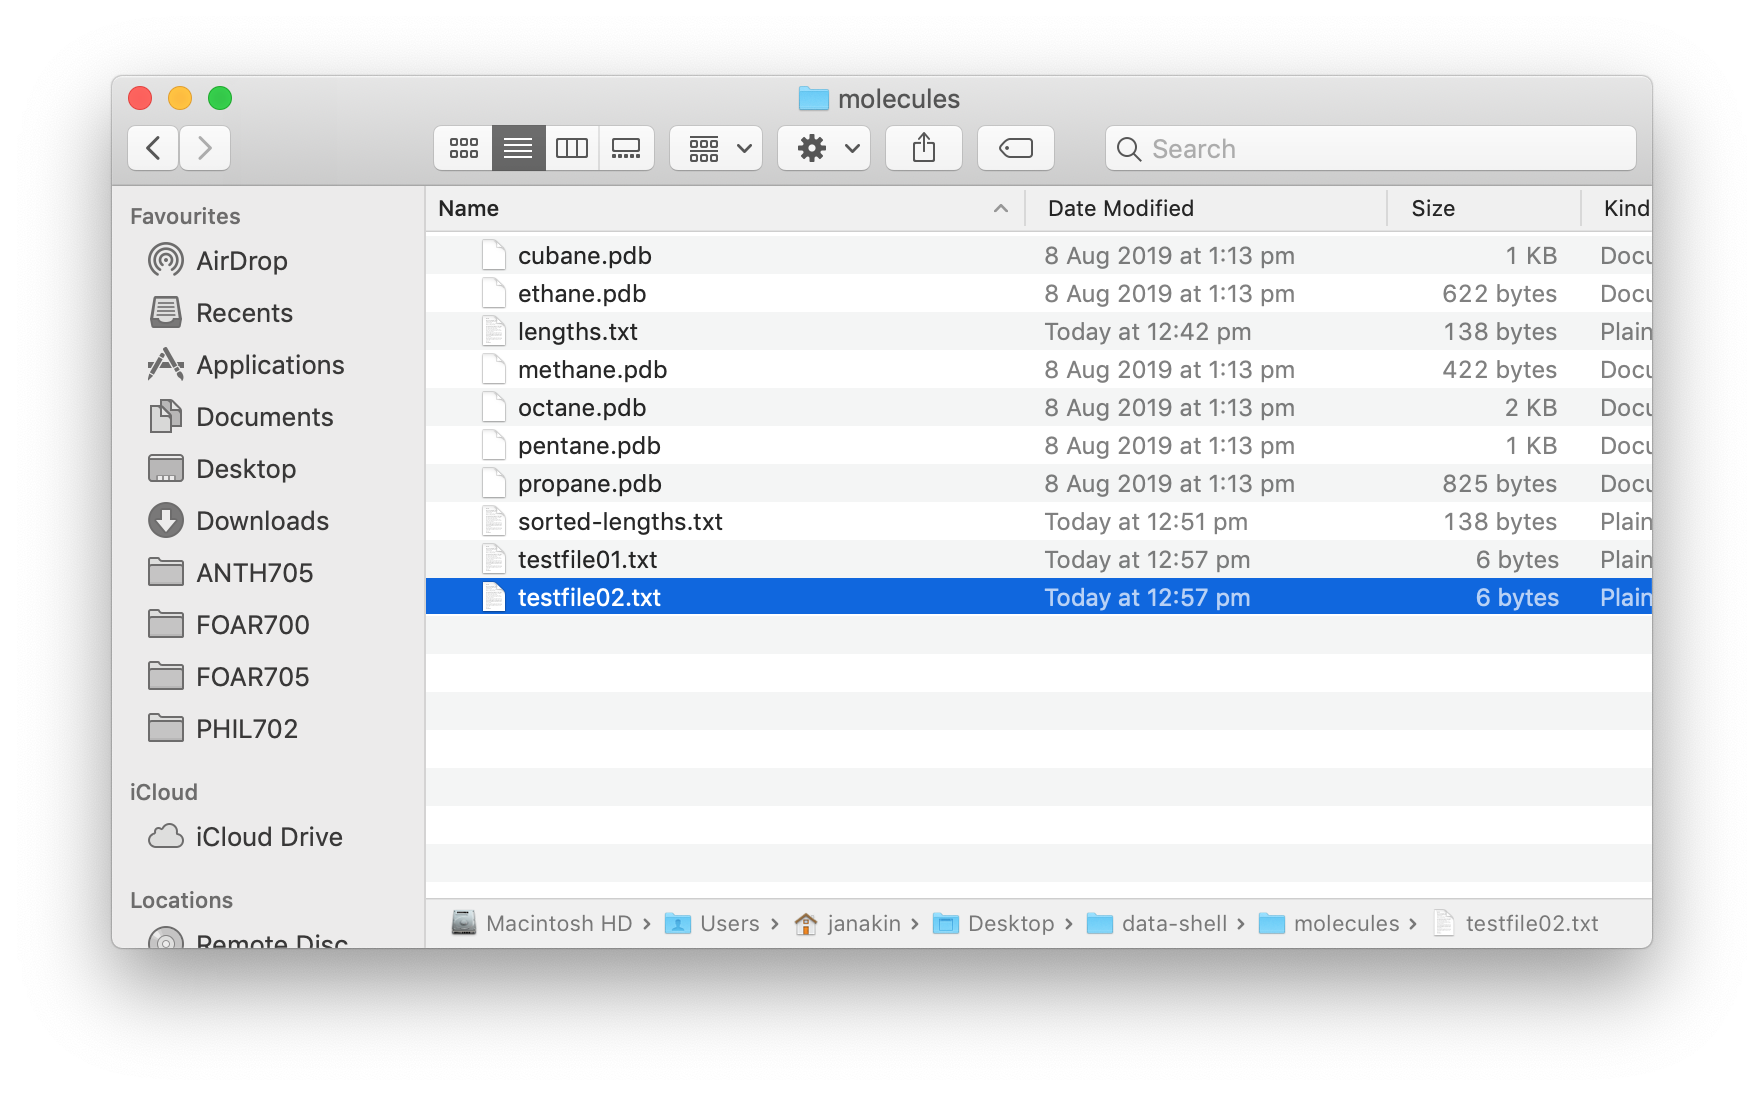
\includegraphics[width=\textwidth]{figh.png}

\section*{4/9/19 - 12:58pm}

The \textit{Appending Data} exercise.

Answer 3. It contains the first three lines and last 2 lines.

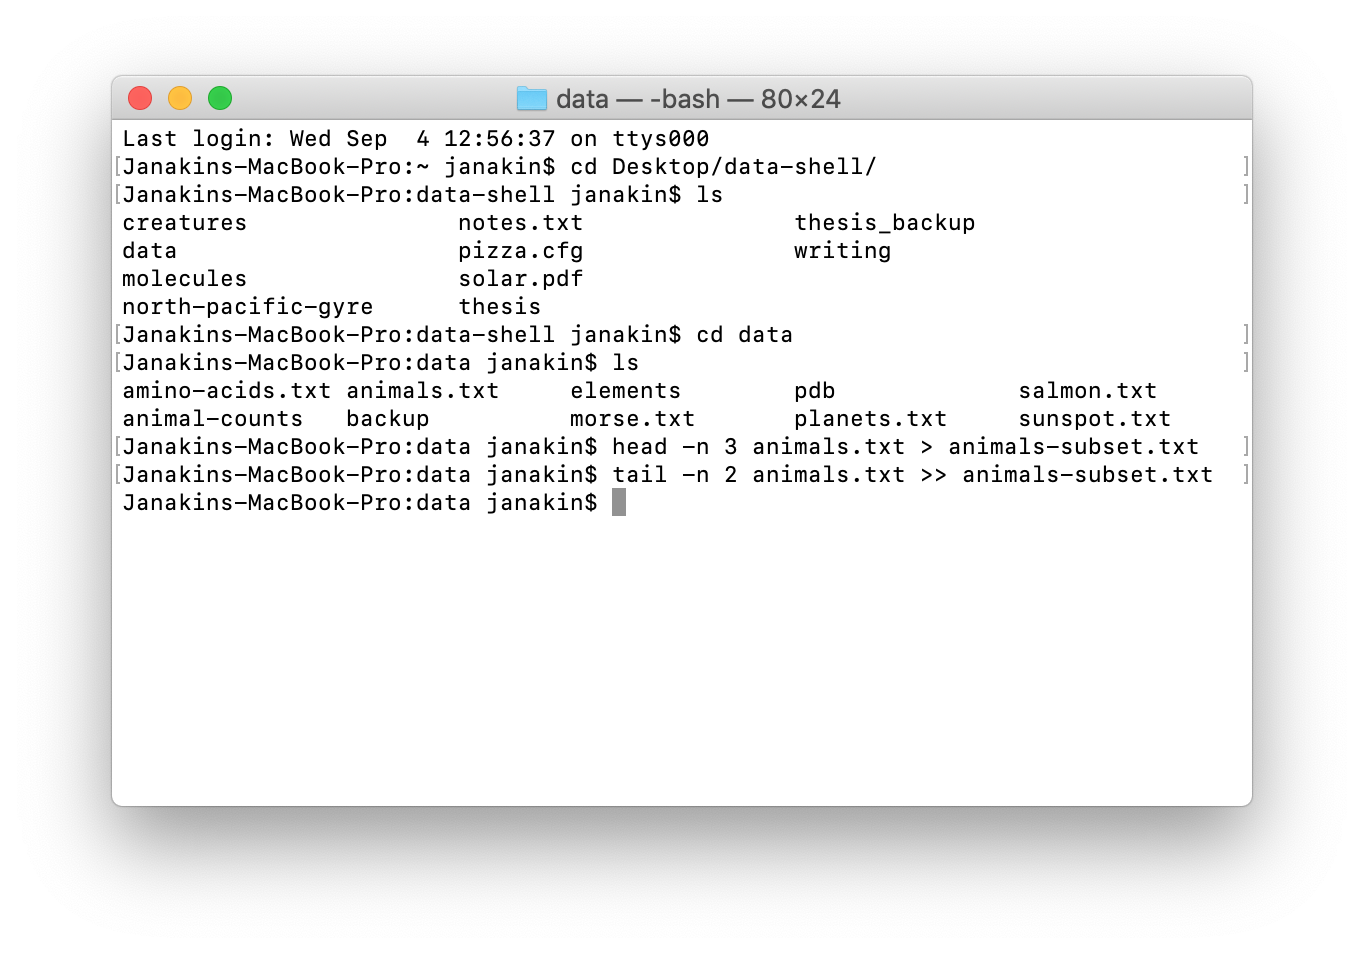
\includegraphics[width=\textwidth]{figi.png}

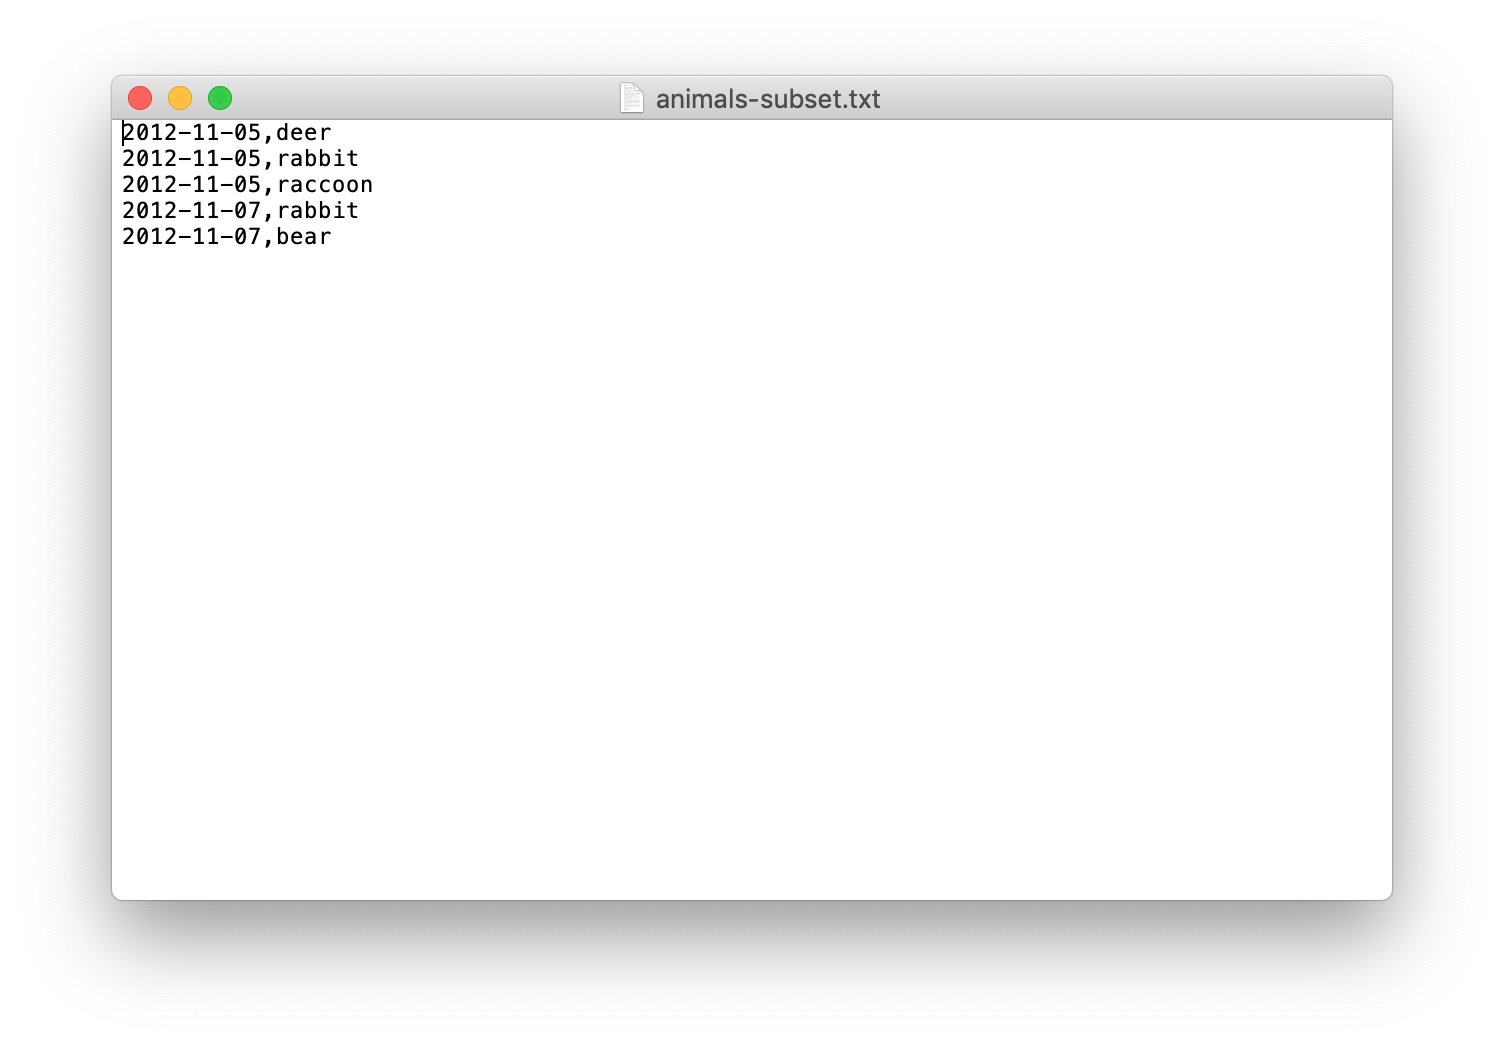
\includegraphics[width=\textwidth]{figj.png}

\section*{4/9/19 - 1:11pm}

Having a go at piping.

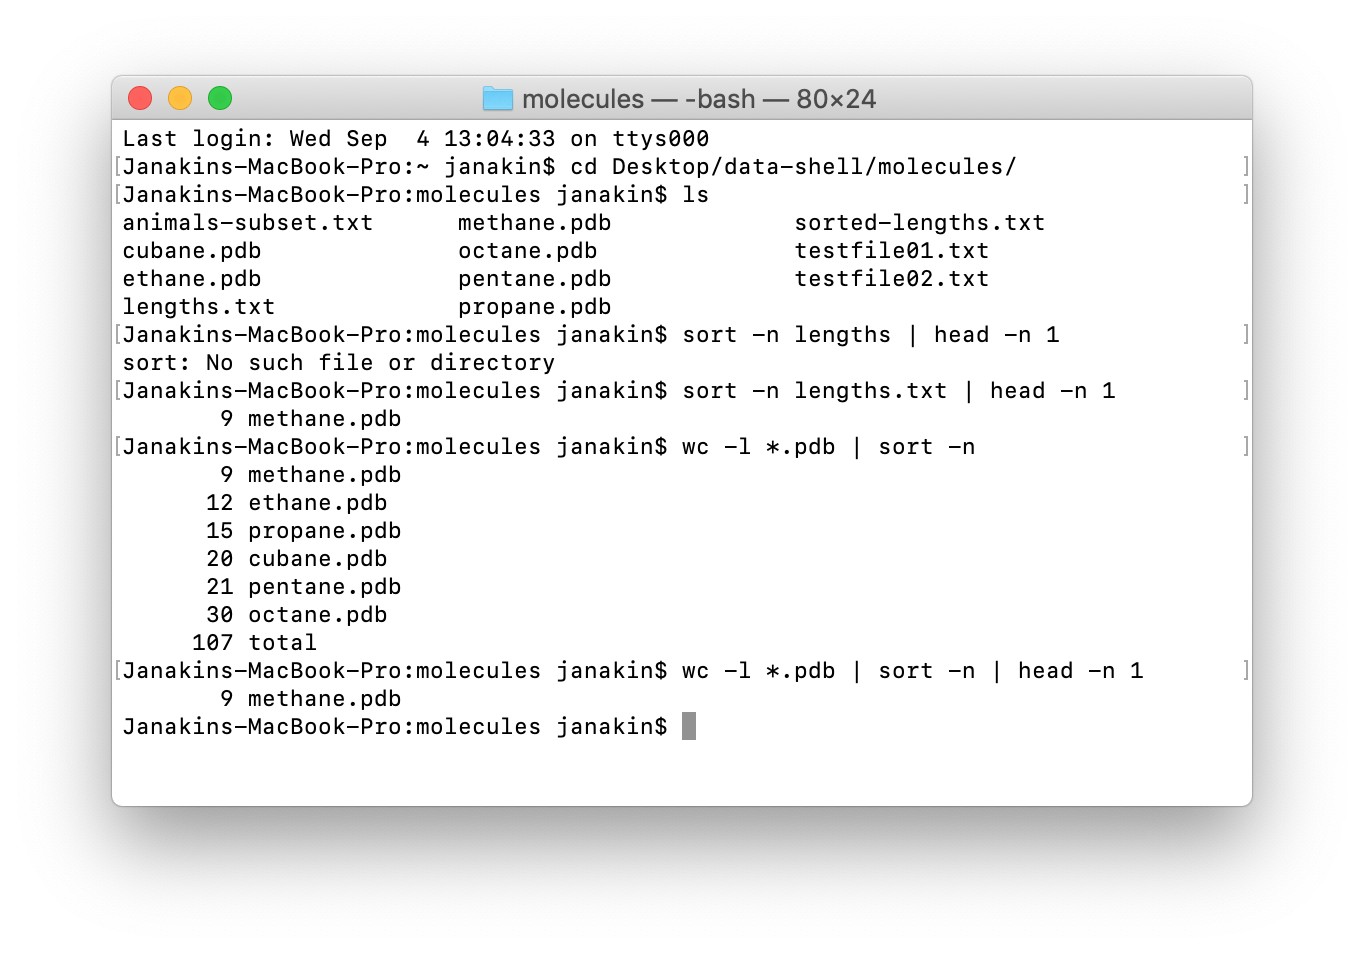
\includegraphics[width=\textwidth]{figk.png}

\section*{4/9/19 - 1:13pm}

\textit{Piping Commands Together} exercise.

The answer is option 4. \begin{verbatim}
    wc -l * | sort -n | head -n 3
\end{verbatim} will get us 3 files which have the least number of lines.

\section*{4/9/19 - 1:15pm}

\textit{Pipe Reading Comprehension} exercise.

As expected, I had the same answer as the exercise.

\begin{verbatim}
2012-11-06,rabbit
2012-11-06,deer
2012-11-05,raccoon
\end{verbatim}

\section*{4/9/19 - 1:19pm}

\textit{Pipe Construction} exercise.

The solution is \begin{verbatim}
    cut -d , -f 2 animals.txt | sort | uniq
\end{verbatim}

\section*{4/9/19 - 1:21pm}

\textit{Which Pipe?} exercise.

The solution is \begin{verbatim}
    cut -d, -f 2 animals.txt | sort | uniq -c | wc -l
\end{verbatim}

\section*{4/9/19 - 1:25pm}

Continuing with Nelle's examples.

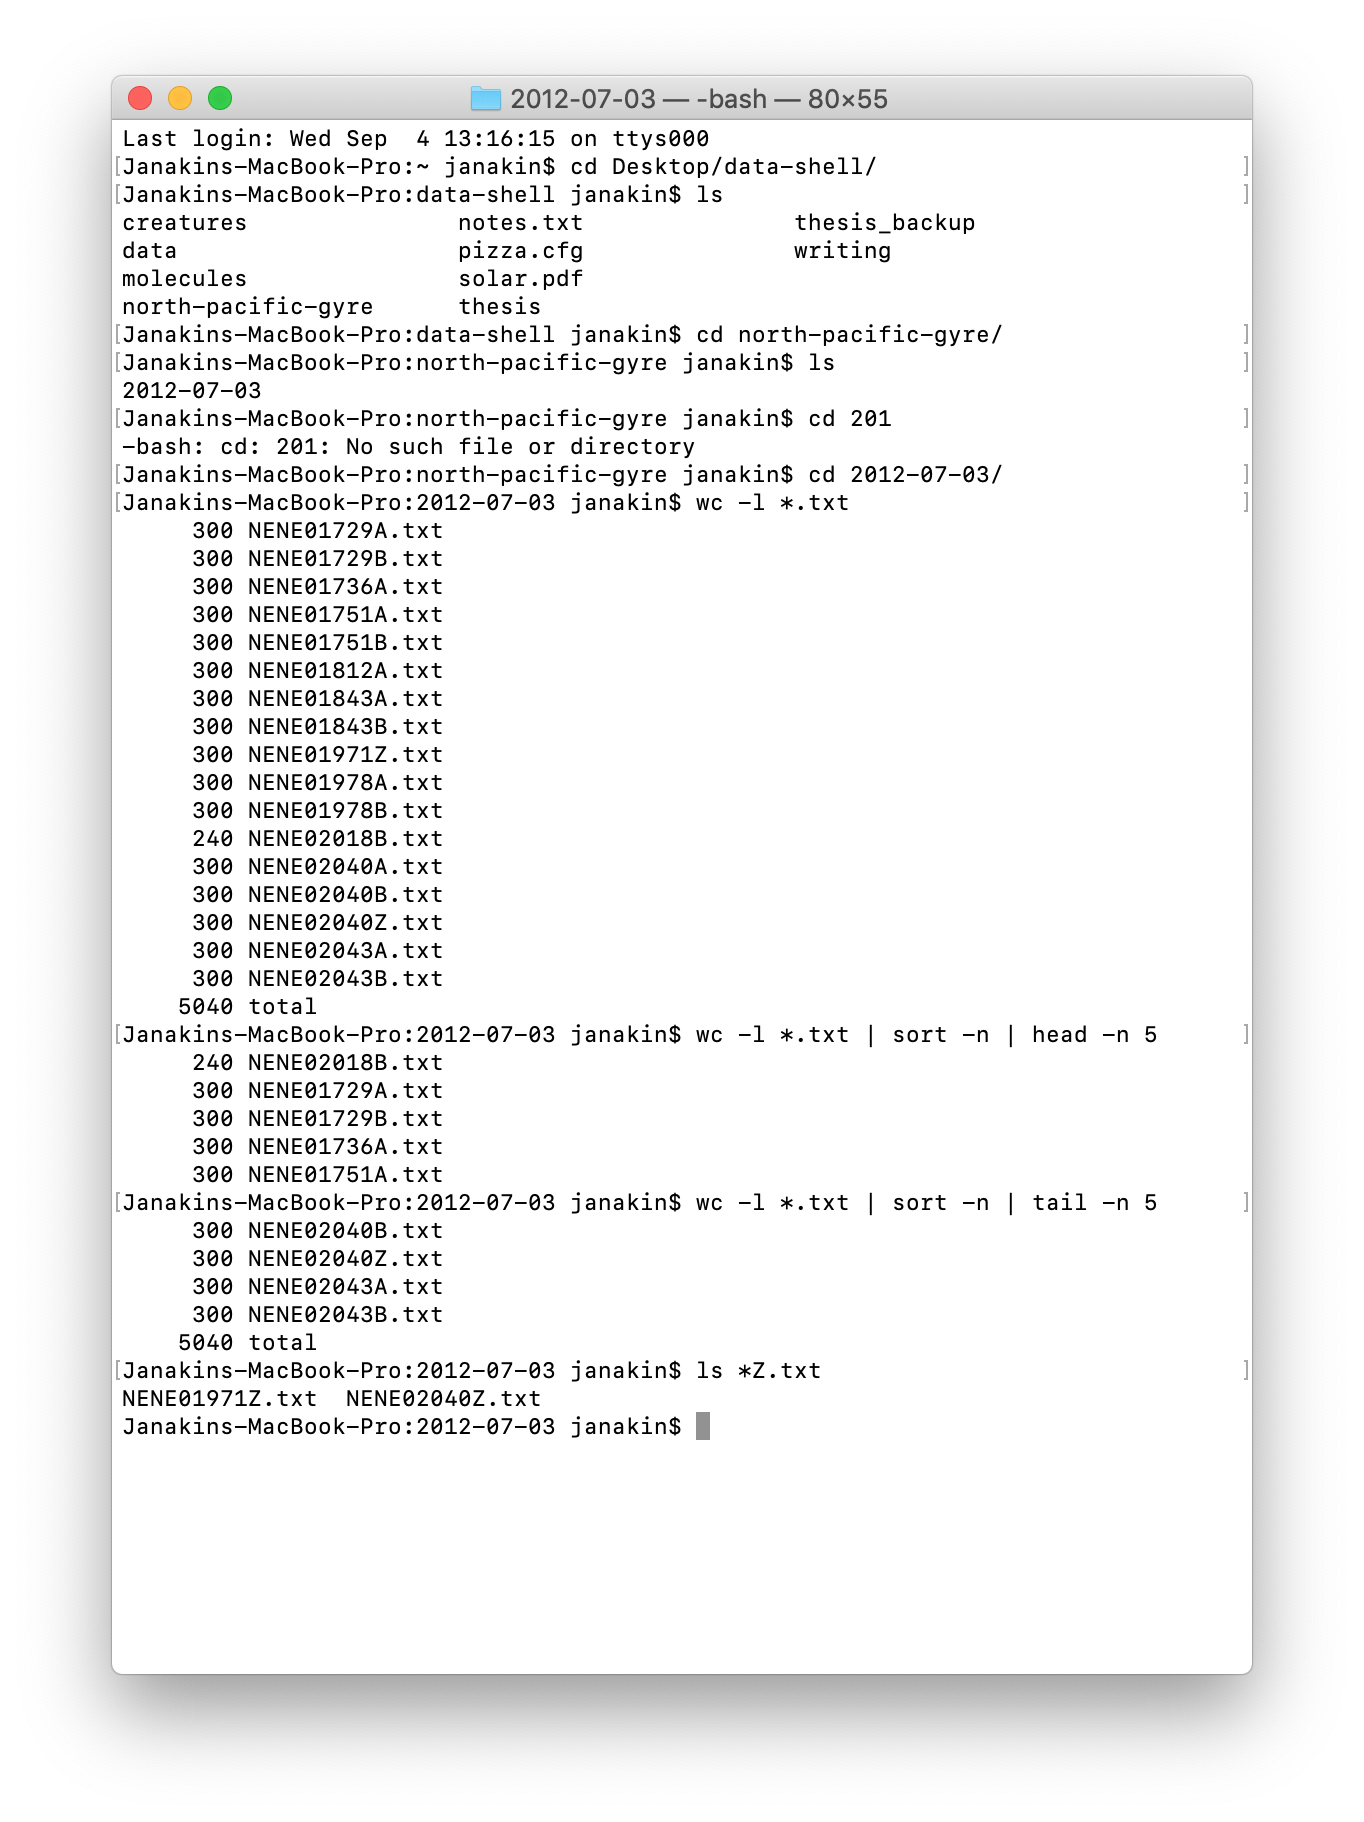
\includegraphics[width=\textwidth]{figl.png}

\section*{4/9/19 - 1:27pm}

\textit{Wildcard Expressions} exercise.

Answers.

\begin{enumerate}
    \item \begin{verbatim}
         ls *A.txt
         ls *B.txt
    \end{verbatim}
    \item They are separated because they are two commands
    \item Only when there are no files ending in A.txt or B.txt
\end{enumerate}

\section*{4/9/19 - 1:31pm}

\textit{Removing Unneeded Files} exercise.

Only \begin{verbatim}
    rm *.txt
\end{verbatim} is correct.

\section*{4/9/19 - 2:08pm}

On to episode 5, \textbf{Loops}. Following the instruction, I had realised that I put in the code \begin{verbatim}
    for filename in basilisk.dat minotaur.dat unicorn.dat
    > do
    >    head -n 2 $filename | tail -n 1
    > done
\end{verbatim} as one continuous code. I then realised that each line was a separate command input.

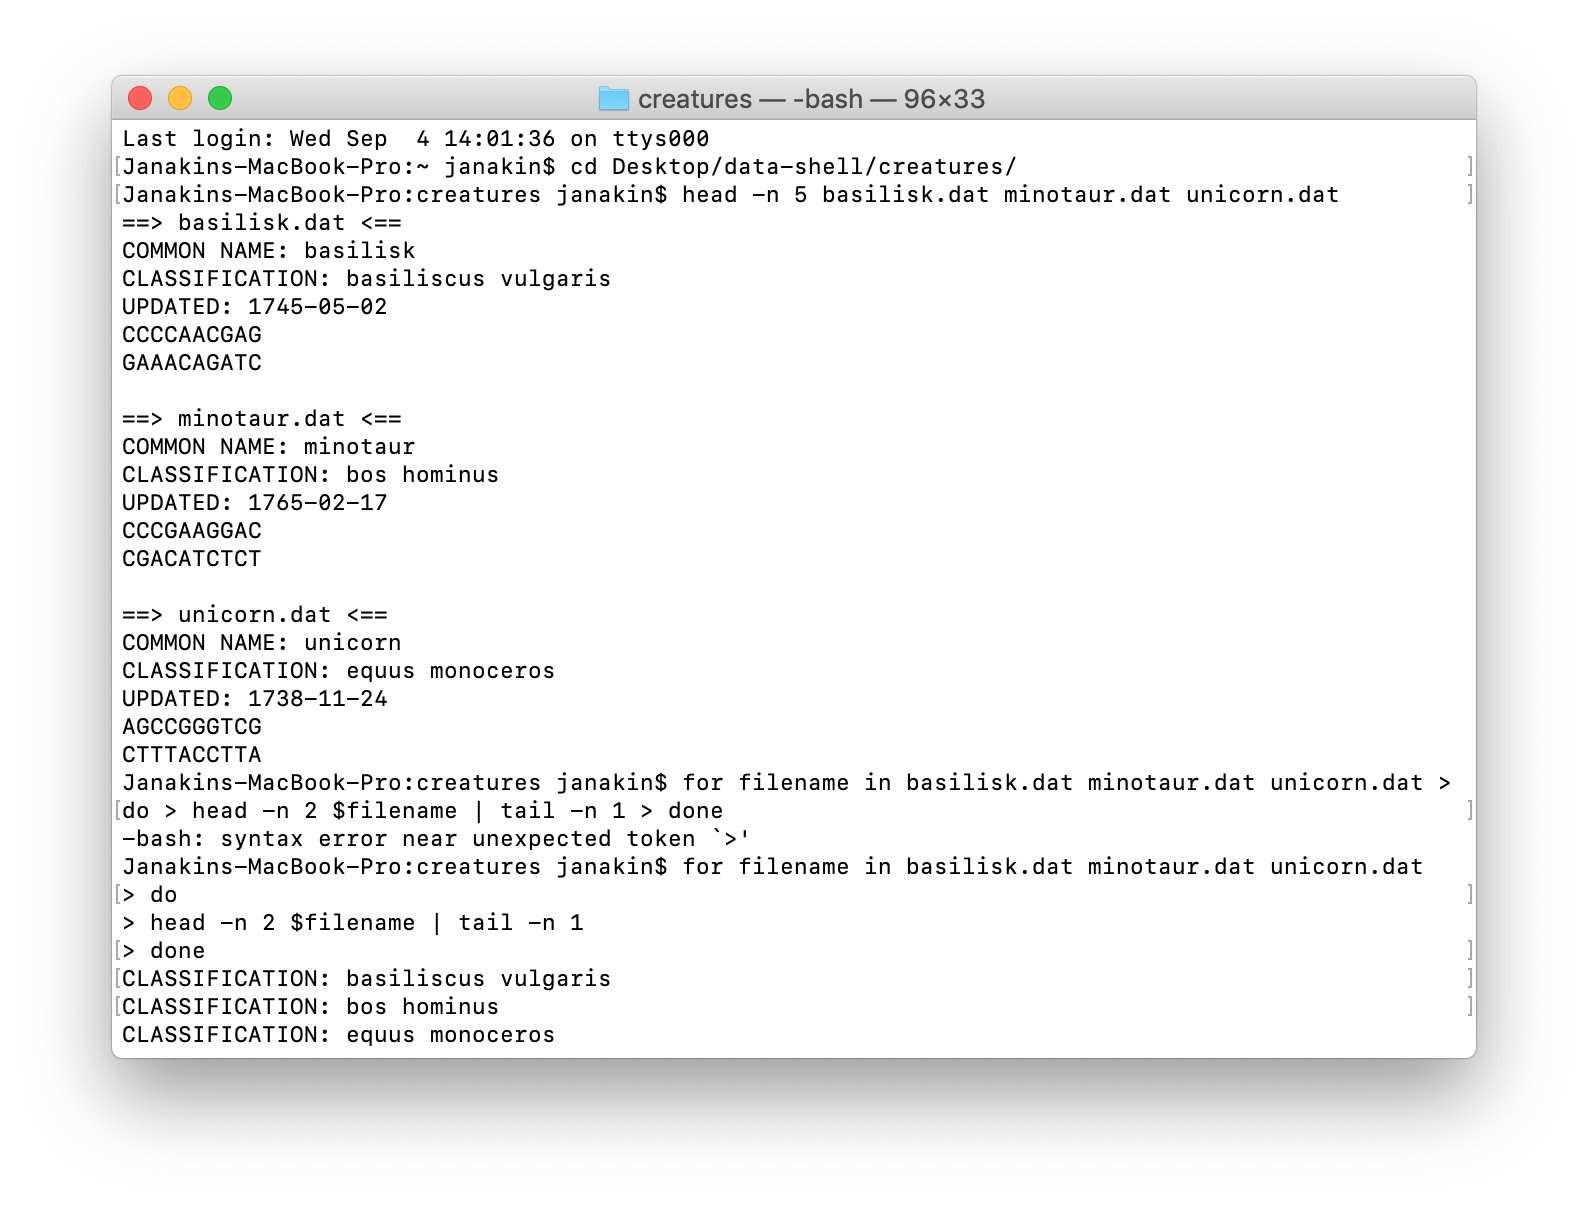
\includegraphics[width=\textwidth]{figm.png}

\section*{4/9/19 - 2:22pm}

Completing \textit{Variables in Loops} exercise. The output of code \begin{verbatim}
    $ for datafile in *.pdb
    > do
    >    ls *.pdb
    > done
\end{verbatim} is

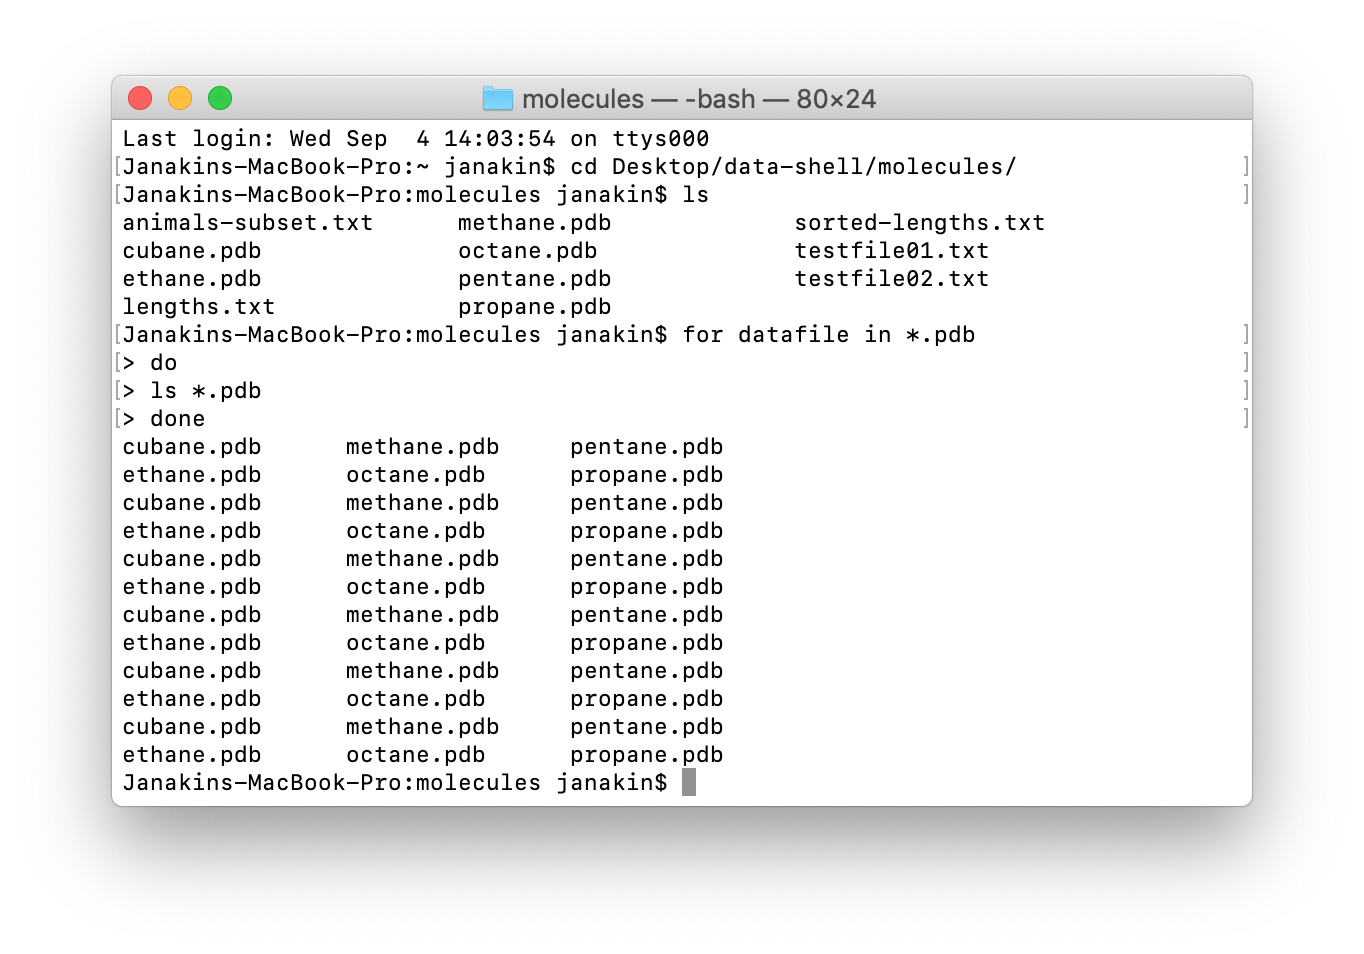
\includegraphics[width=\textwidth]{fign.png}

The output code of \begin{verbatim}
    $ for datafile in *.pdb
    > do
    >	ls $datafile
    > done
\end{verbatim} is

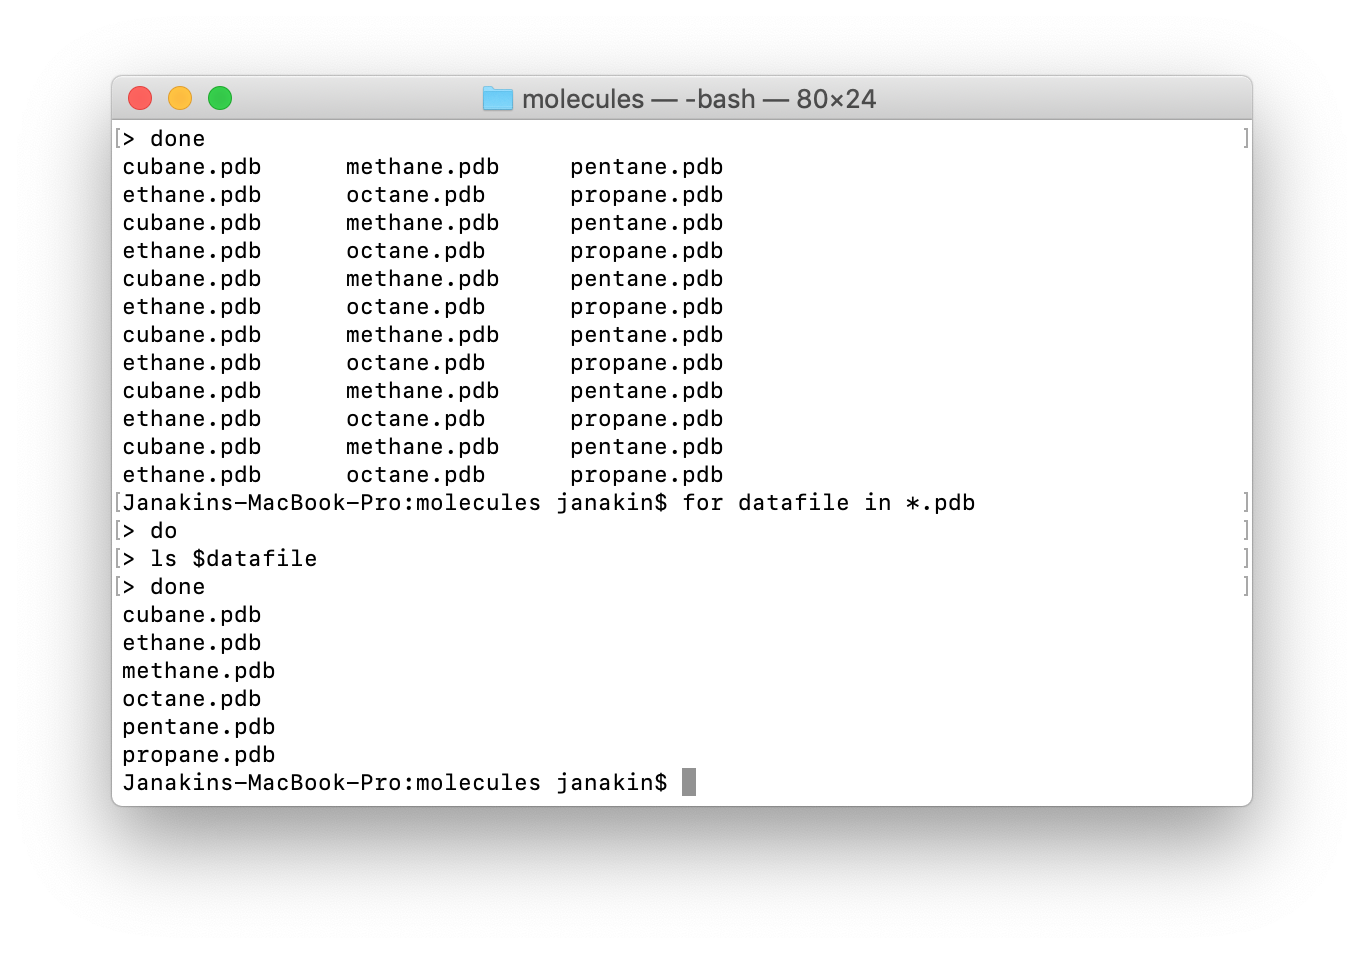
\includegraphics[width=\textwidth]{figo.png}

The second code lists a different file on each loop iteration.

\section*{4/9/19 - 2:28pm}

Completing \textit{Limiting Sets of Files} exercise.

\begin{verbatim}
    $ for filename in c*
    > do
    >    ls $filename
    > done
\end{verbatim} lists only cubane.pdb.

\begin{verbatim}
    $ for filename in *c*
    > do
    >    ls $filename
    > done
\end{verbatim} lists both cubane.pdb and octane.pdb because of the presence of the c character.

\section*{4/9/19 - 2:32pm}

Completing \textit{Saving to a File in a Loop - Part One} exercise.

\begin{verbatim}
    for alkanes in *.pdb
    do
    echo $alkanes
    cat $alkanes > alkanes.pdb
    done
\end{verbatim} has text from each file written into aklanes.pdb. Each iteration overwrites the last. The propane.pdb is the last to be written in alkanes.pdb.

\section*{4/9/19 - 2:36pm}

Completing \textit{Saving to a File in a Loop - Part Two} exercise.

All of the text from cubane.pdb, ethane.pdb, methane.pdb, octane.pdb, pentane.pdb and propane.pdb would be concatenated and saved to a file called all.pdb.

\section*{4/9/19 - 2:44pm}

Continuing with the lesson.

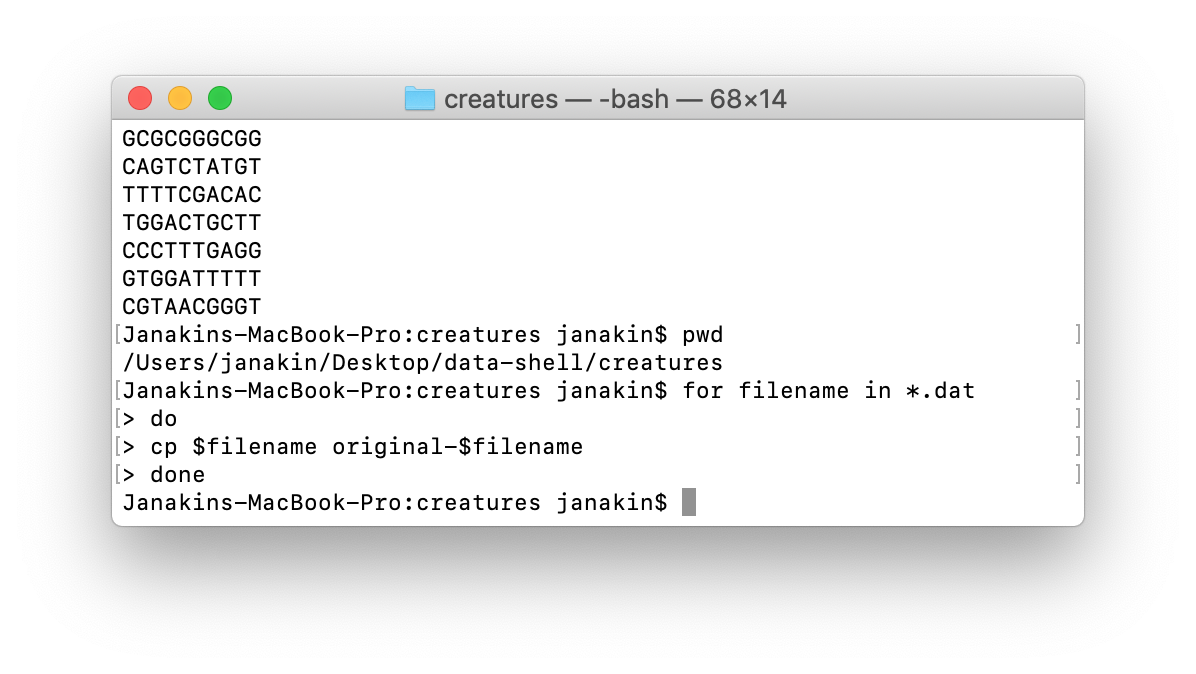
\includegraphics[width=\textwidth]{figp.png}

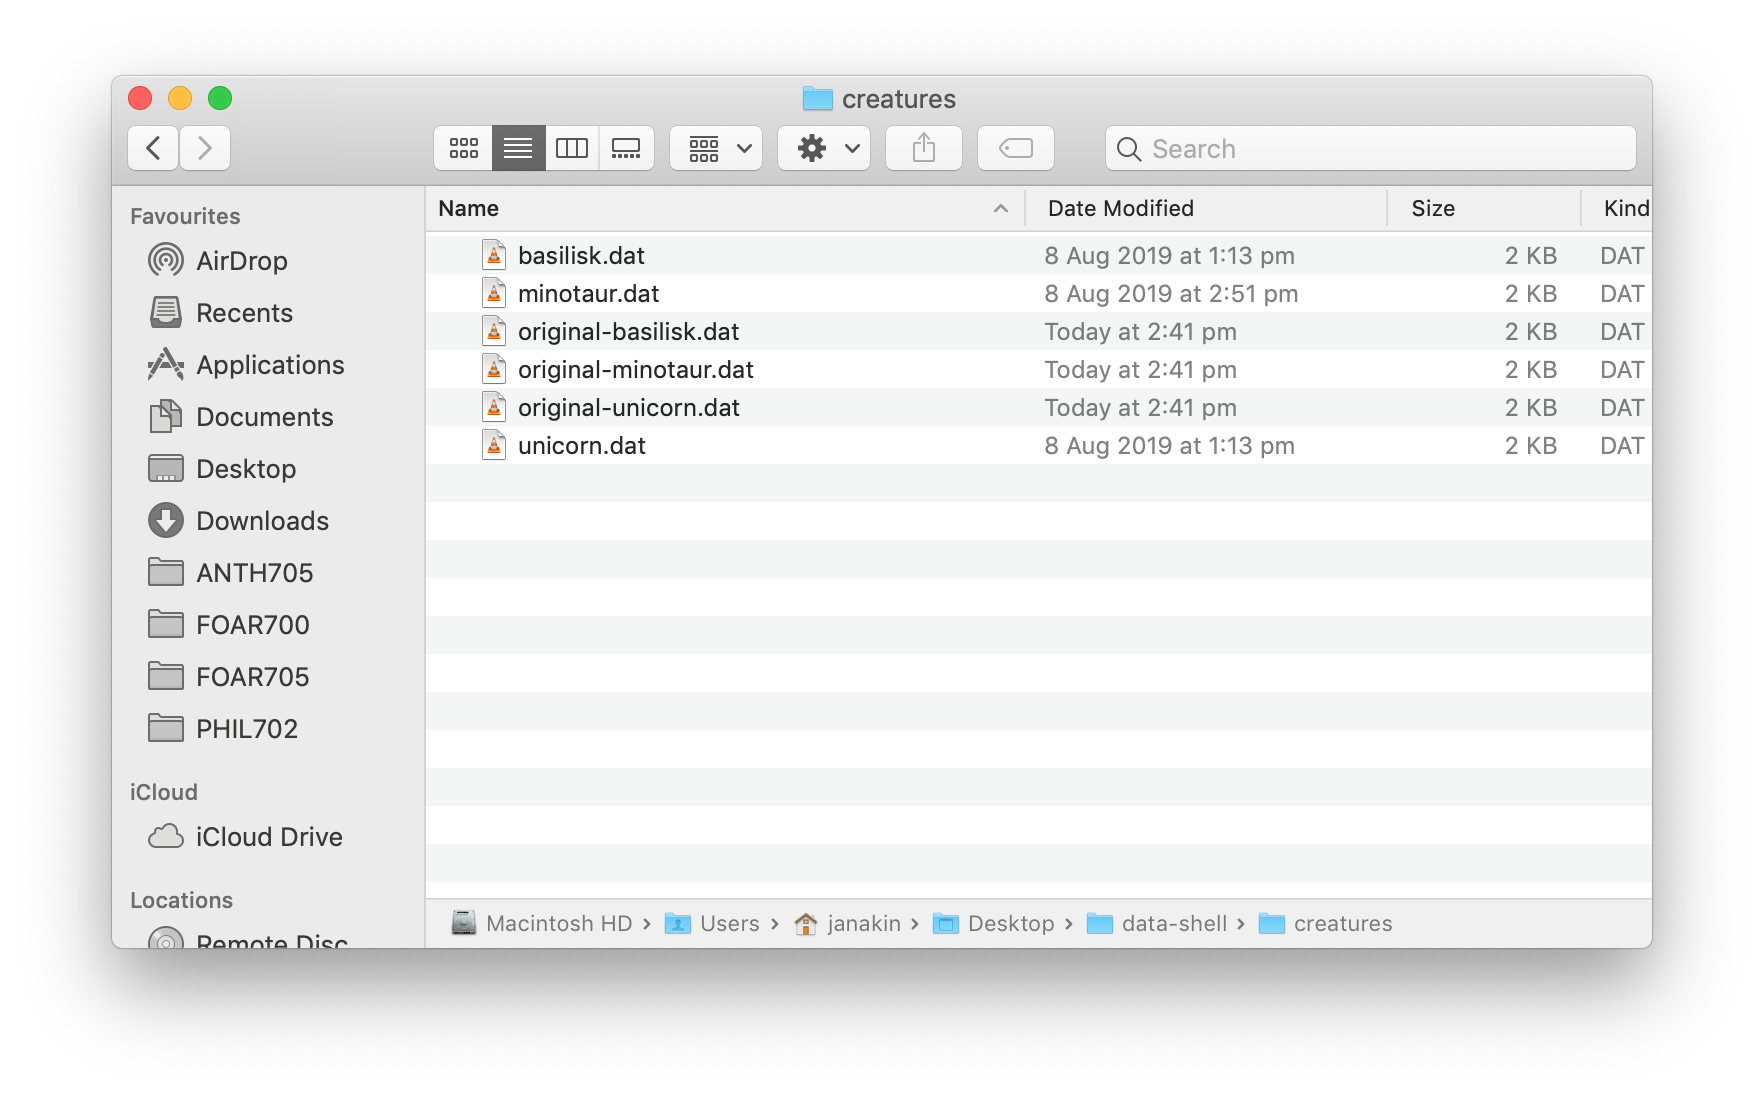
\includegraphics[width=\textwidth]{figq.png}

\section*{4/9/19 - 2:53pm}

Back with Nelle's example.

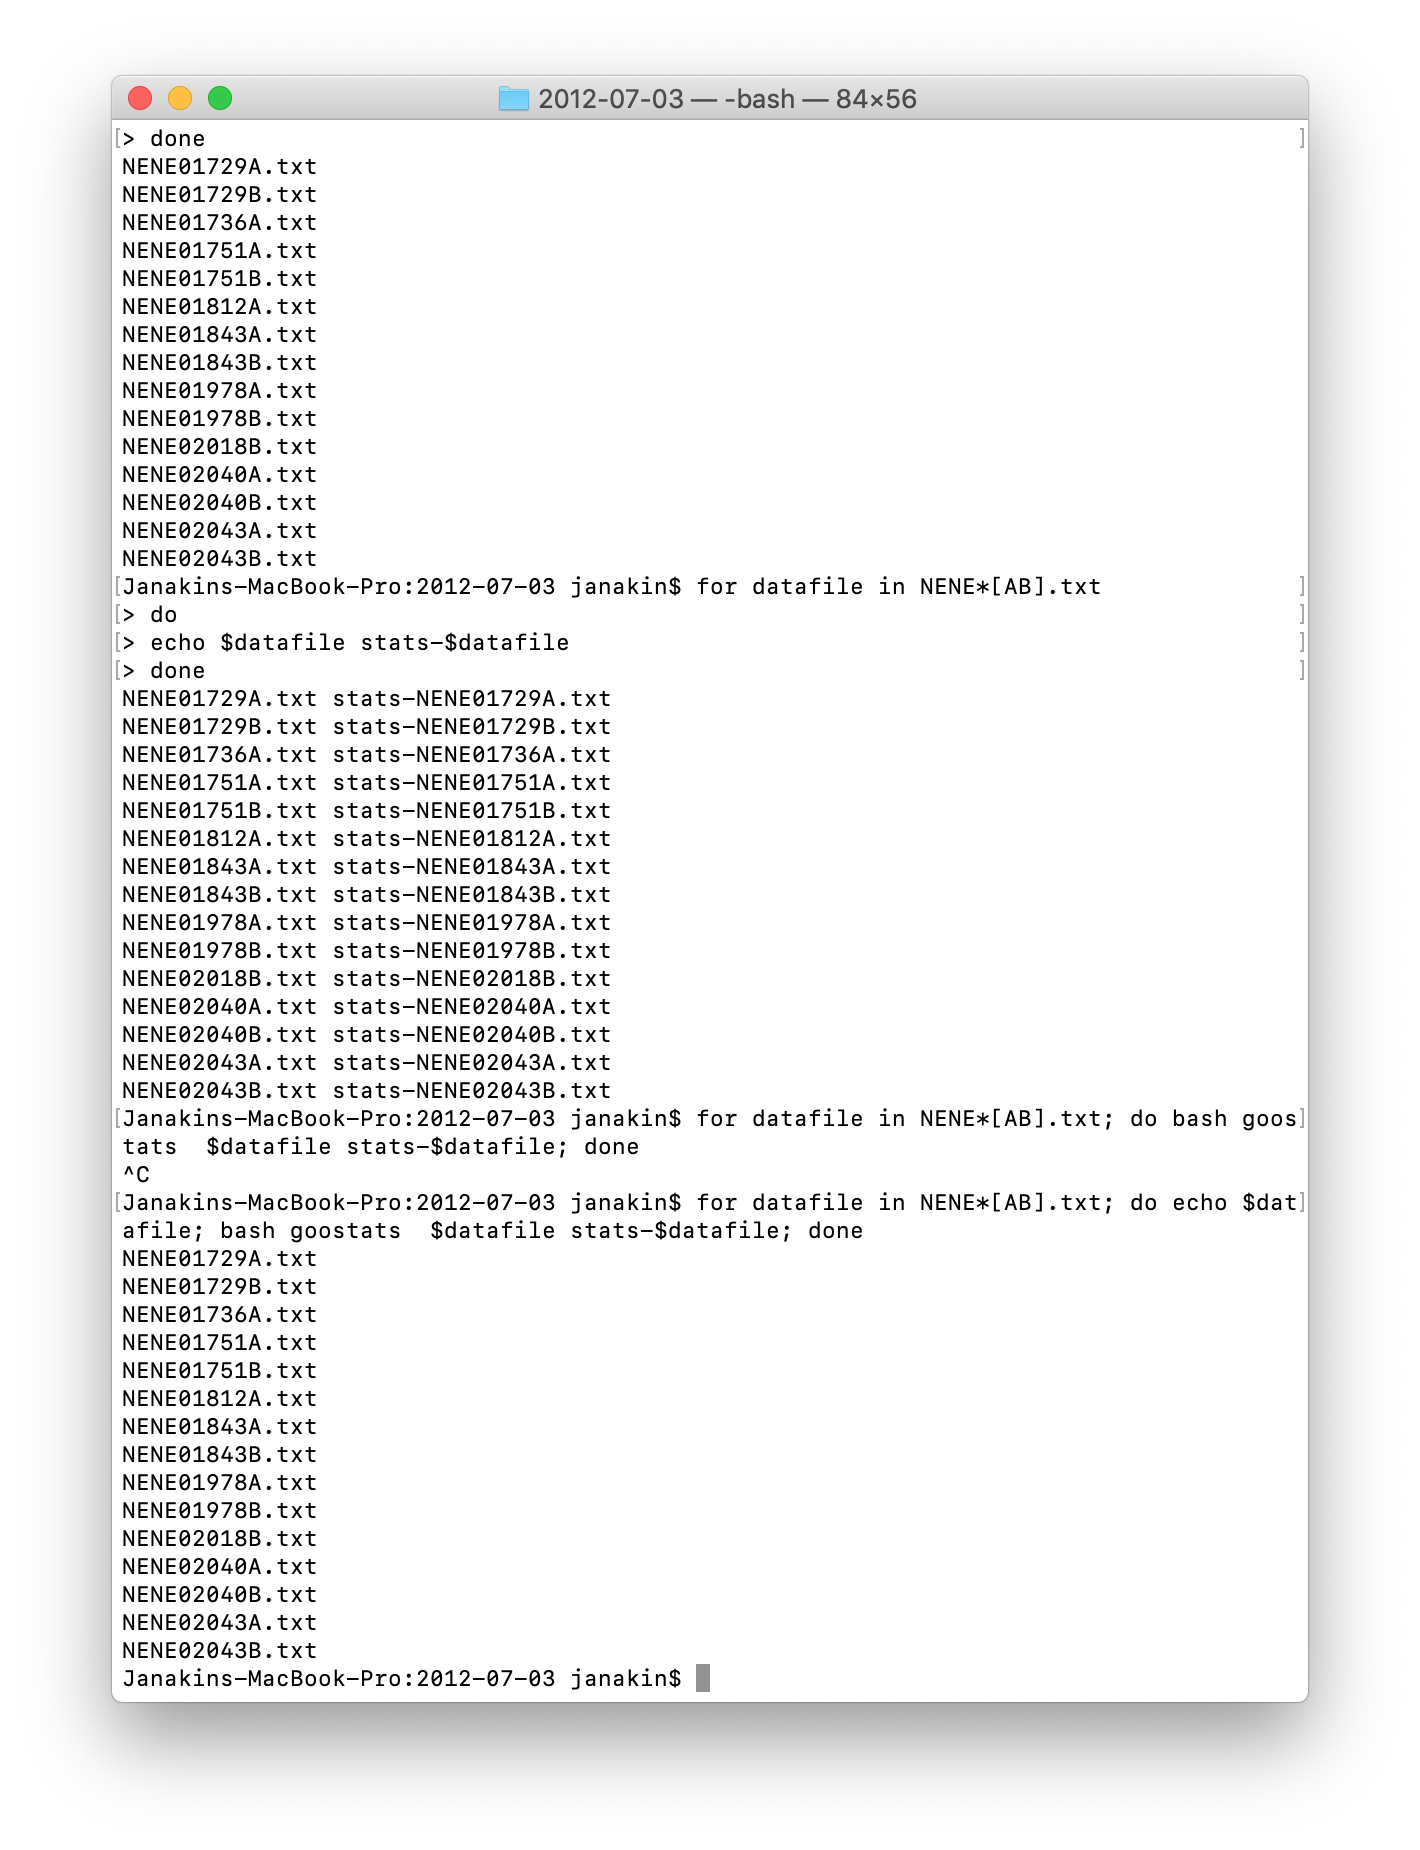
\includegraphics[width=\textwidth]{figr.png}

Not exactly sure what bash goostats did, but it did certainly look like Terminal was doing something.

\section*{4/9/19 - 2:59pm}

Completing \textit{Doing a Dry Run} exercise.

The second version is the one we want to run because it prints everything.

\section*{4/9/19 - 3:03pm}

Completing \textit{Nested Loops} exercise.

Not sure if this was successful.

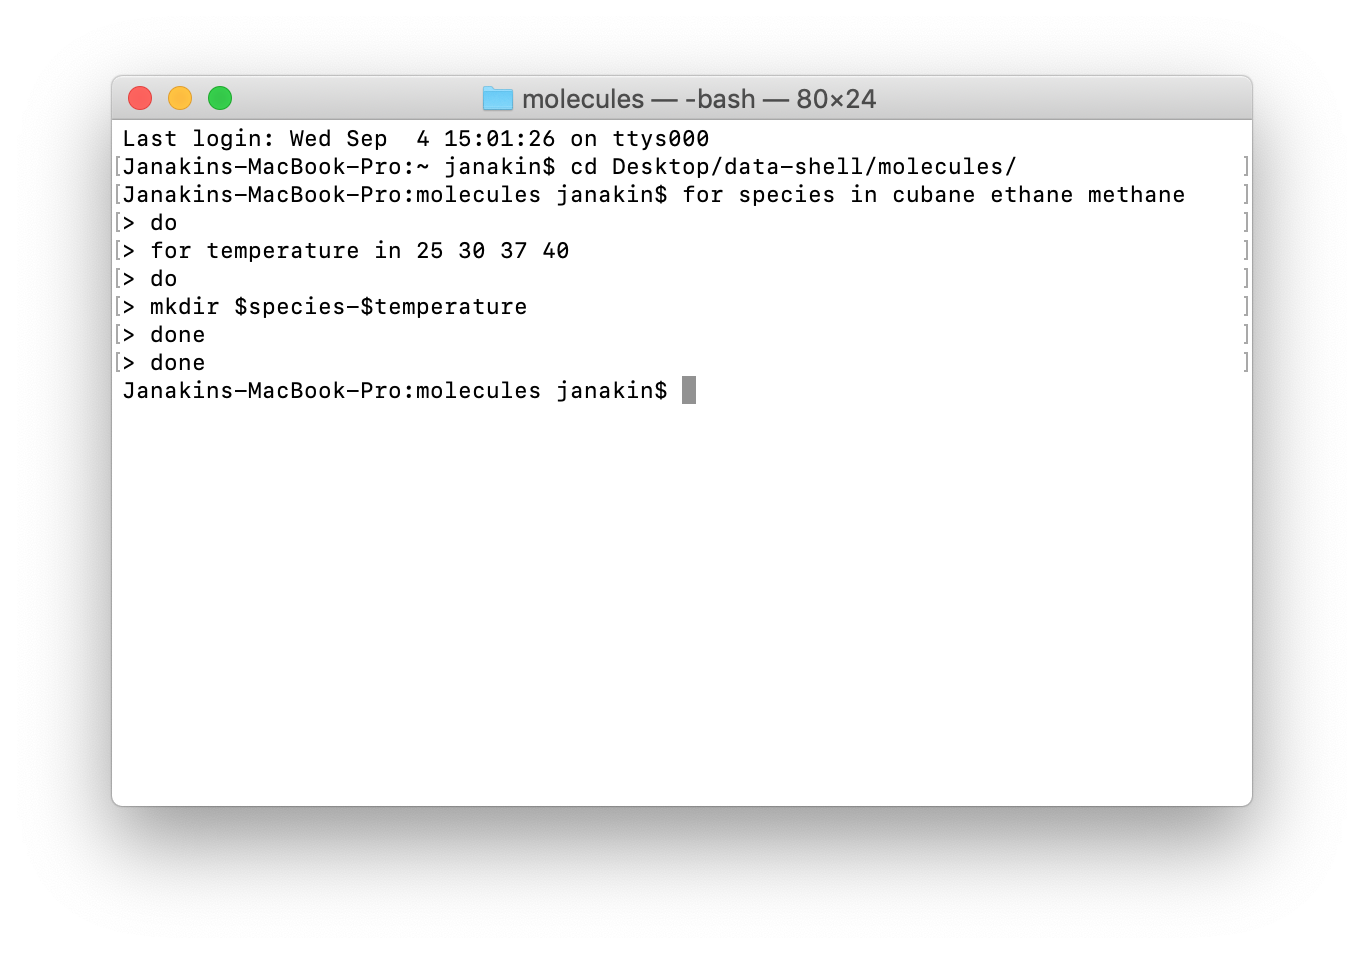
\includegraphics[width=\textwidth]{figs.png}

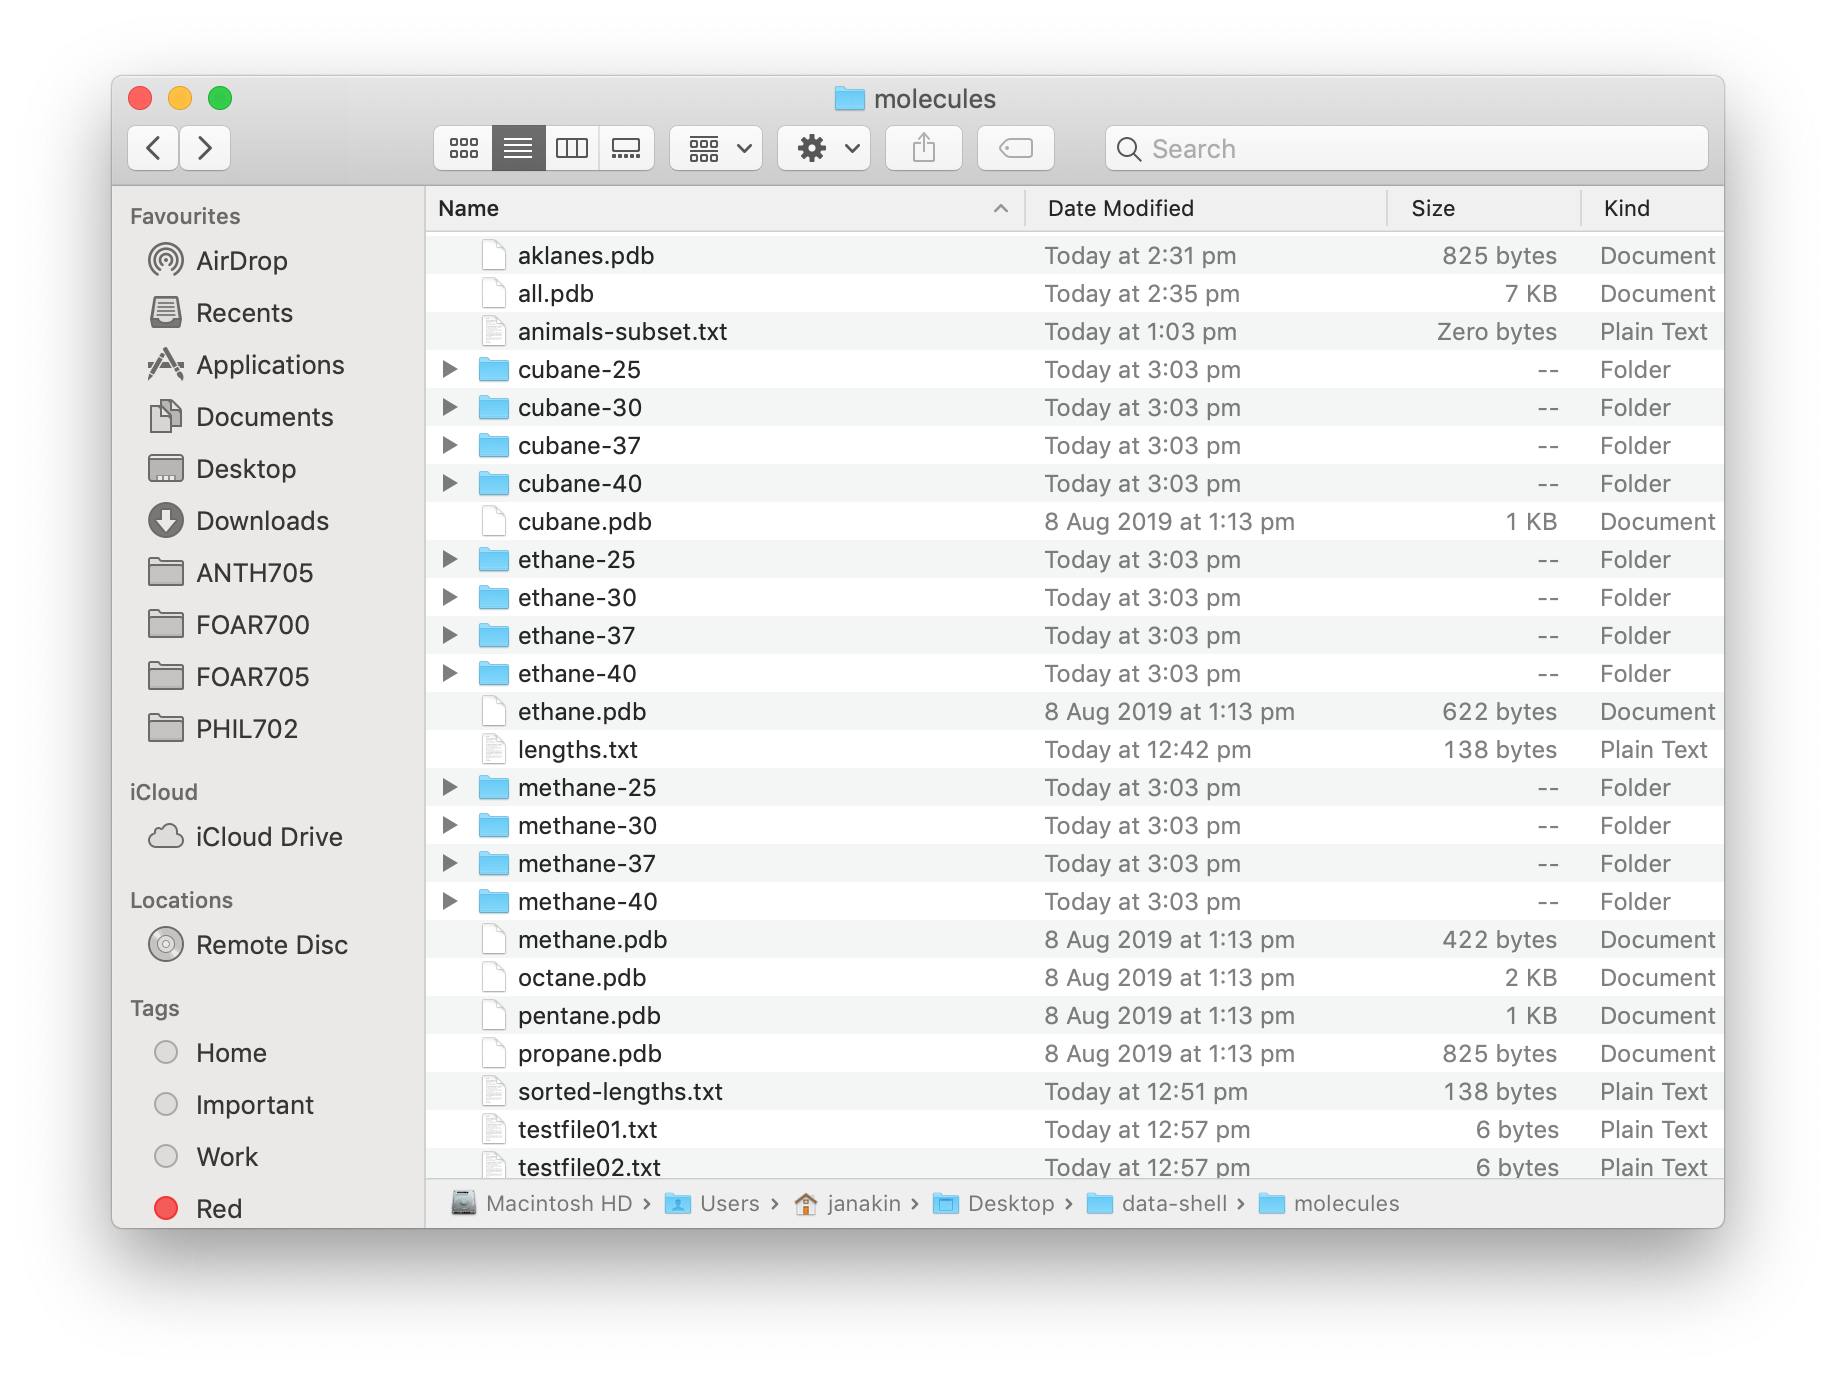
\includegraphics[width=\textwidth]{figt.png}

\section*{4/9/19 - 3:16pm}

\textbf{Episode 6: Shell Scripts}

Following the instructions. Below are the screenshots of what I have done.

Creating the middle.sh shell.

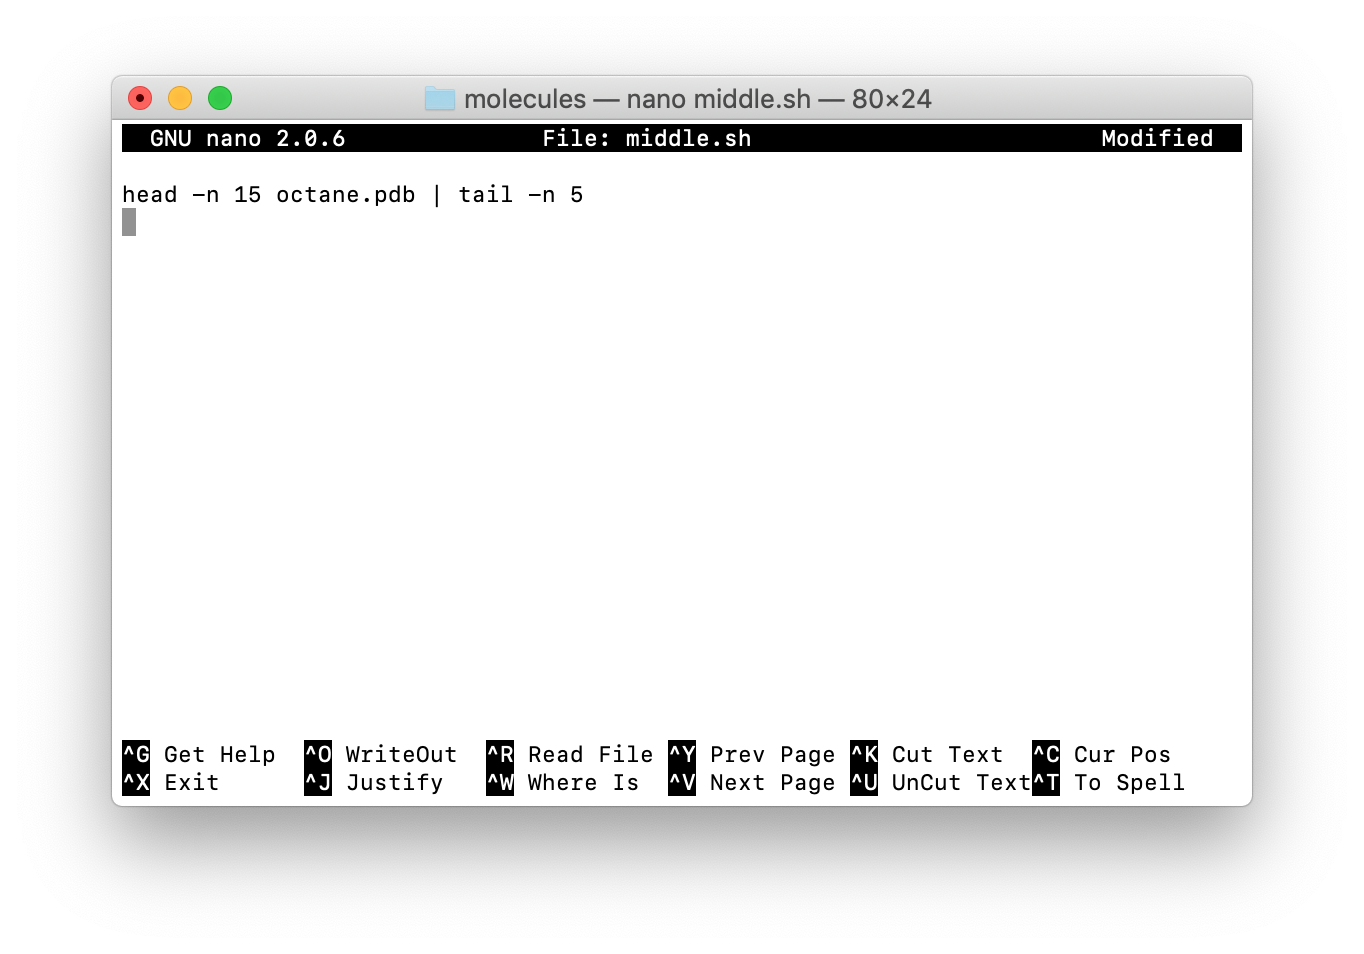
\includegraphics[width=\textwidth]{figu.png}

Recoded the middle.sh file to be more versatile and include information to other users about what it does.

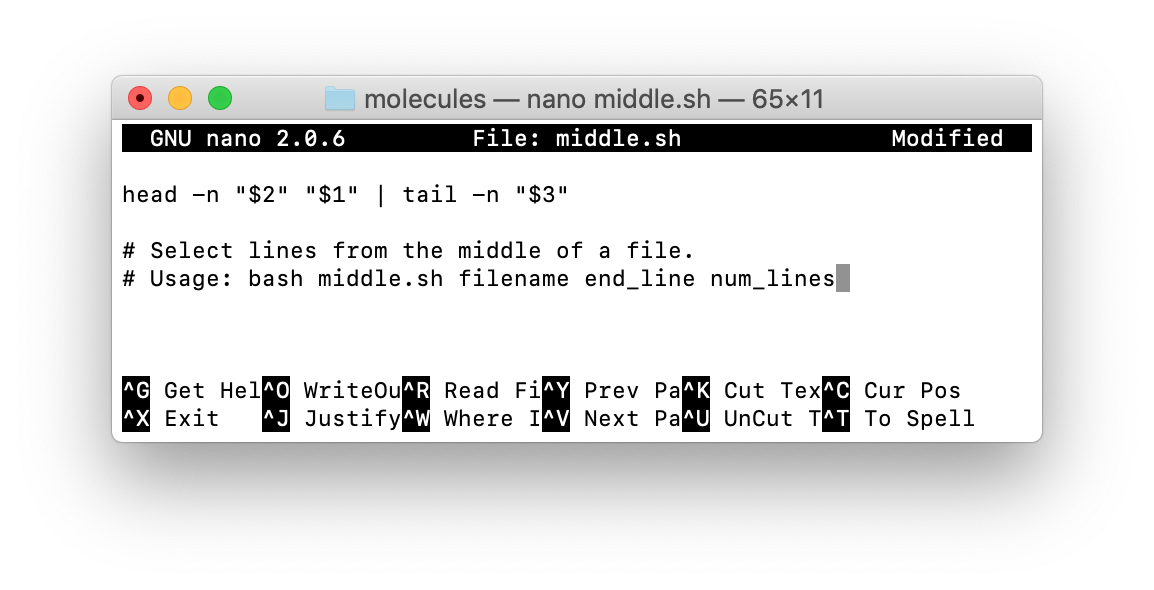
\includegraphics[width=\textwidth]{figv.png}

Created the sorted.sh shell.

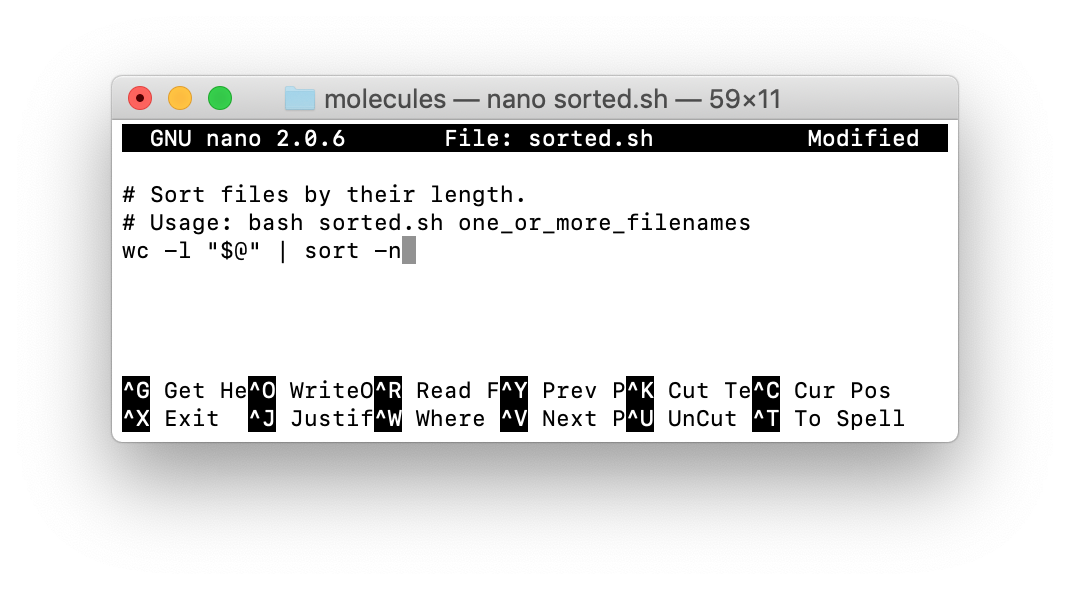
\includegraphics[width=\textwidth]{figw.png}

Terminal window and commands used up until this point.

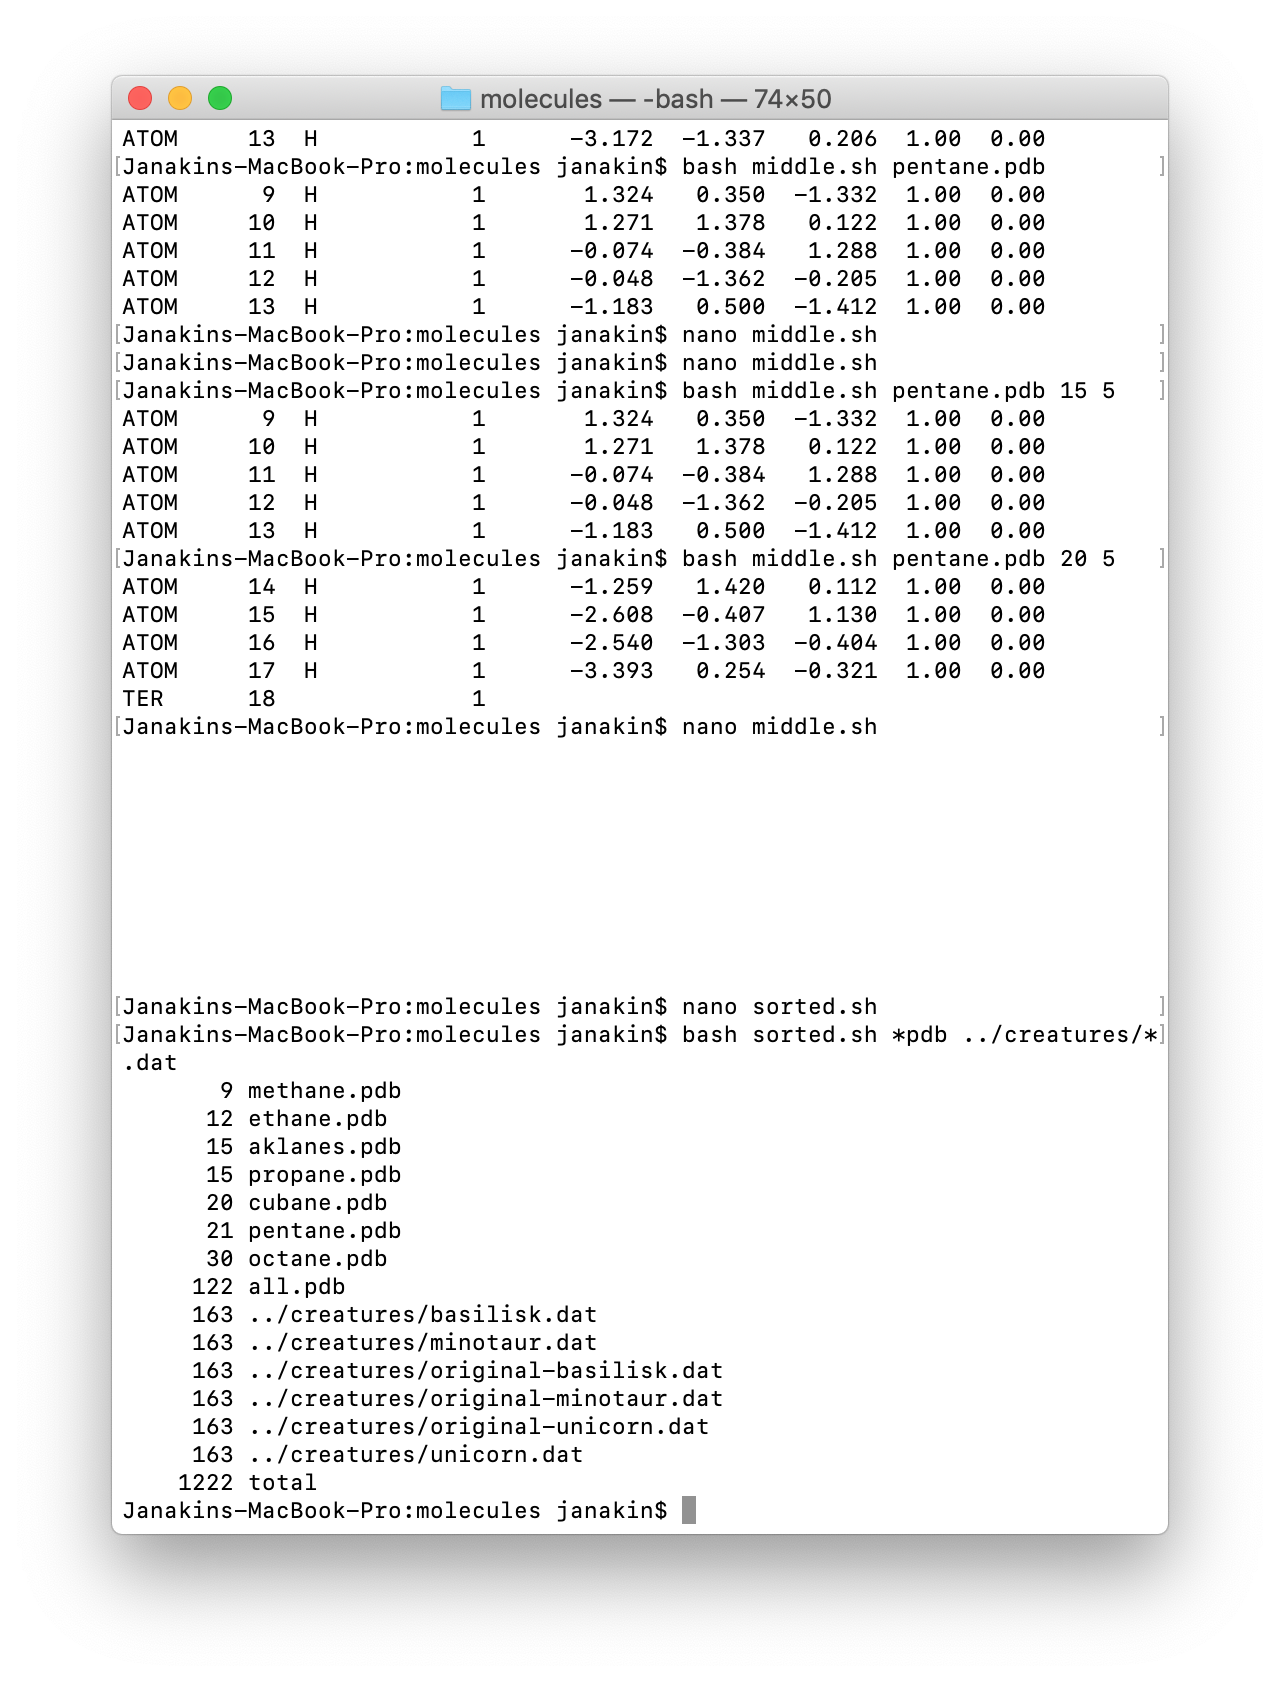
\includegraphics[width=\textwidth]{figx.png}

\section*{4/9/19 - 3:34pm}

\textit{List Unique Species} exercise. The script I would use.

\begin{verbatim}
    for file in $@
    do
	echo "Unique species in $file:"
	# Extract species names
	cut -d , -f 2 $file | sort | uniq
    done
\end{verbatim}

\section*{4/9/19 - 3:36pm}

\textit{Why Record Commands in the History Before Running Them}

It is a good idea to do this because it gives you a record of what commands you used, and in what order. So if things go wrong, you can trouble shoot.

\section*{4/9/19 - 3:41pm}

Following on with Nelle's example.

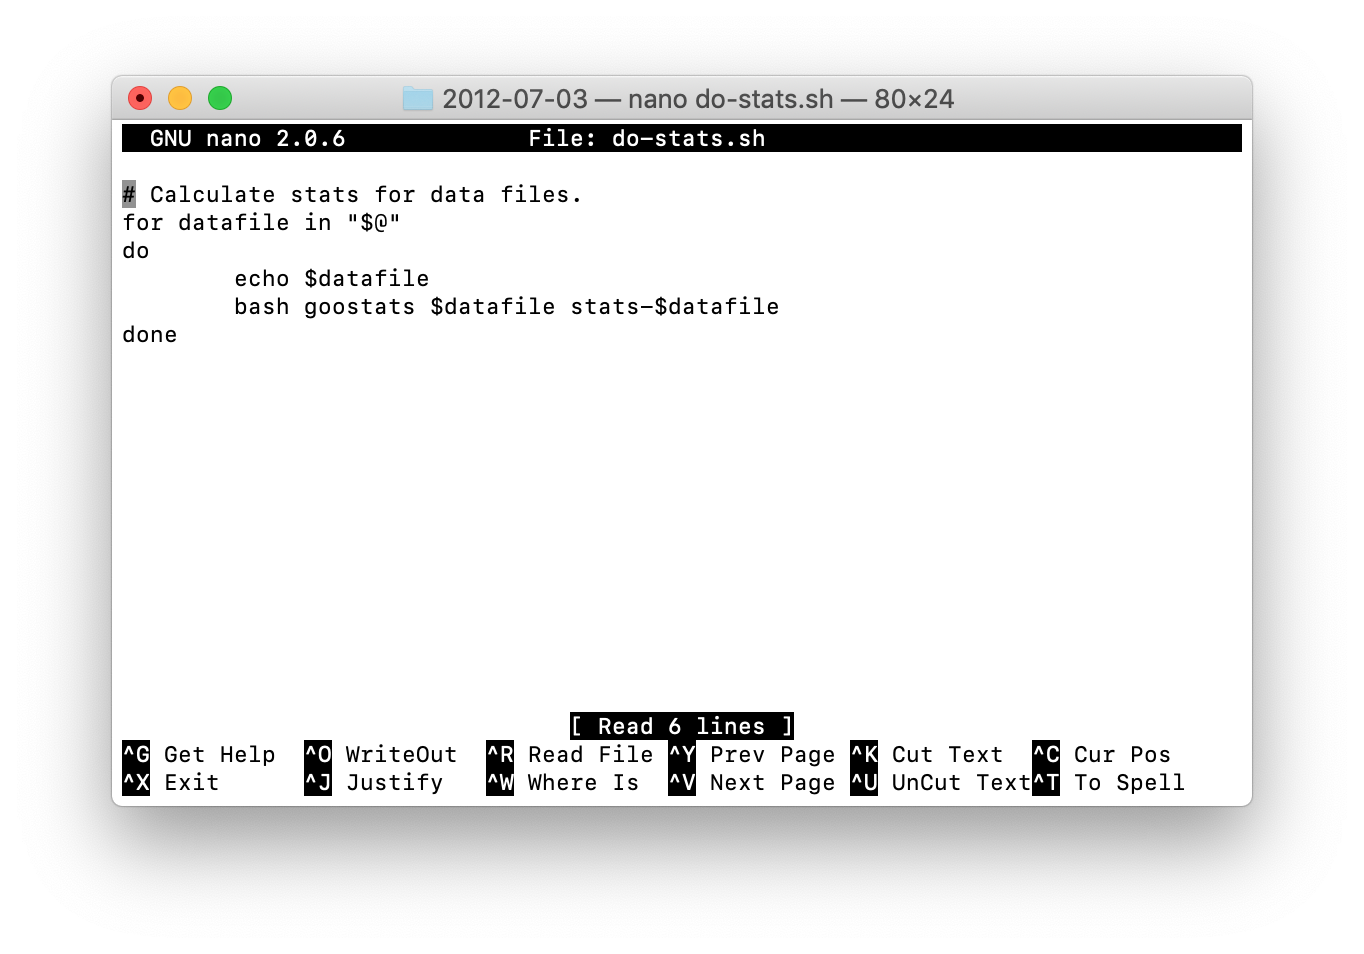
\includegraphics[width=\textwidth]{figy.png}

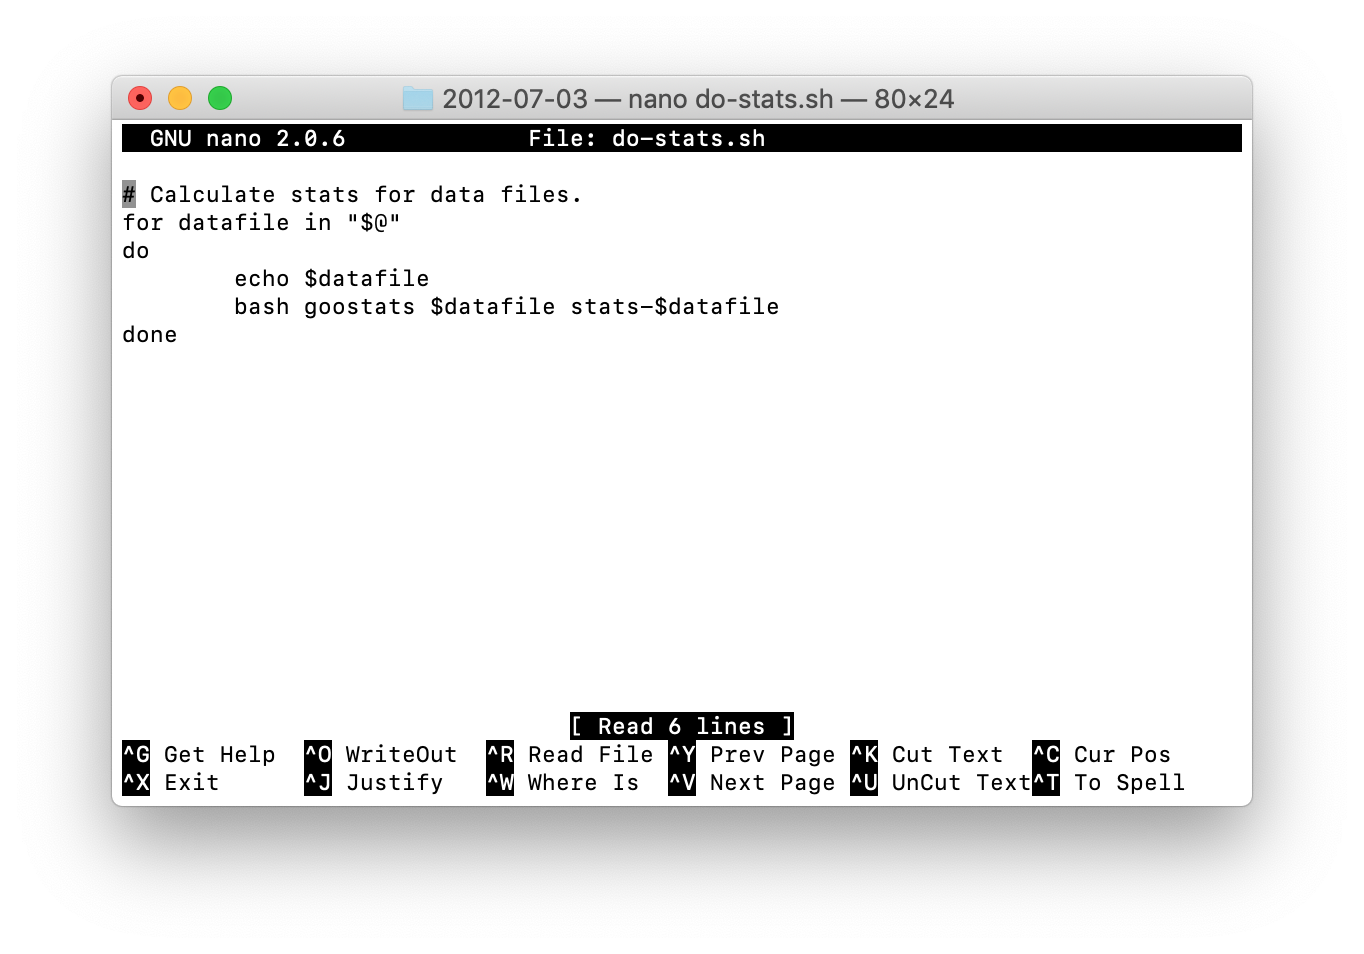
\includegraphics[width=\textwidth]{figz.png}

\section*{4/9/19 - 3:43pm}

\textit{Variables in Shell Scripts}

The correct answer is 2.The first and the last line of each file ending in .pdb in the molecules directory

\section*{4/9/19 - 3:44pm}

\textit{Find the Longest File With a Given Extension}

I would use the code \begin{verbatim}
    wc -l $1/*.$2 | sort -n | tail -n 2 | head -n 1
\end{verbatim}

\section*{4/9/19 - 3:47pm}

\textit{Script Reading Comprehension}

Script 1 would print out a list of all files containing a dot. Script 2 would print the contents of the first 3 files with a .pdb extension. Script 3 would print all the arguments to the script followed by .pdb.

\section*{4/9/19 - 3:48pm}

\textit{Debugging Script}

The -x option gets bash to run in debug mode, printing out each command as it runs it, which will help when trouble shooting.

\section*{4/9/19 - 10:44am}

Am now on the 6th and final episode \textbf{Finding Things}.

The first little bit.

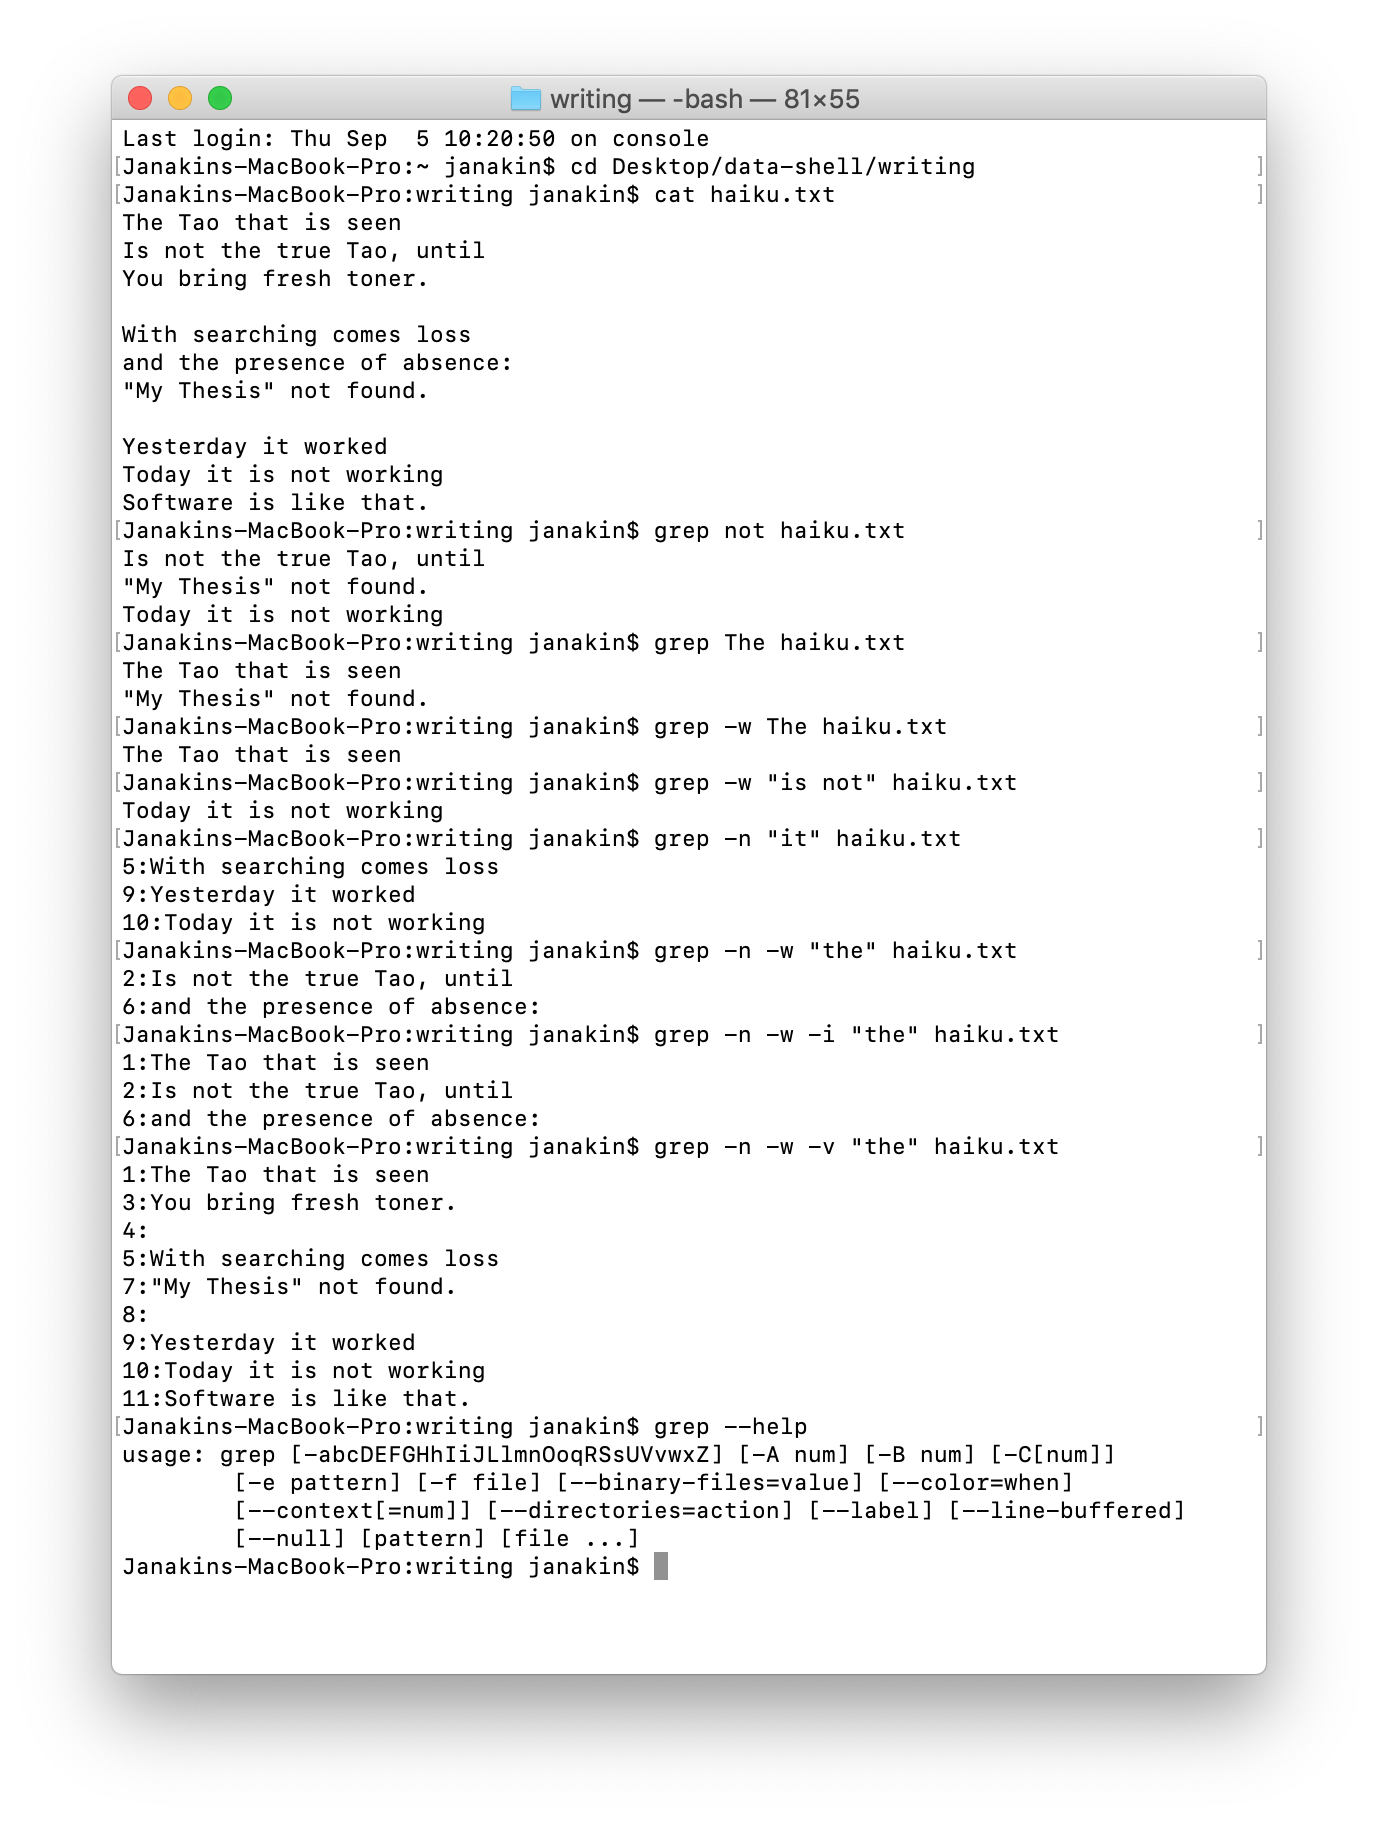
\includegraphics[width=\textwidth]{fta.png}

\section*{4/9/19 - 10:50am}

\textit{Using grep}

The correct answer is 3 \begin{verbatim}
    grep -w "of" haiku.txt
\end{verbatim} because it will only look for whole words.

\section*{4/9/19 - 10:57am}

\textit{Tracking a Species}

I made this shell script.

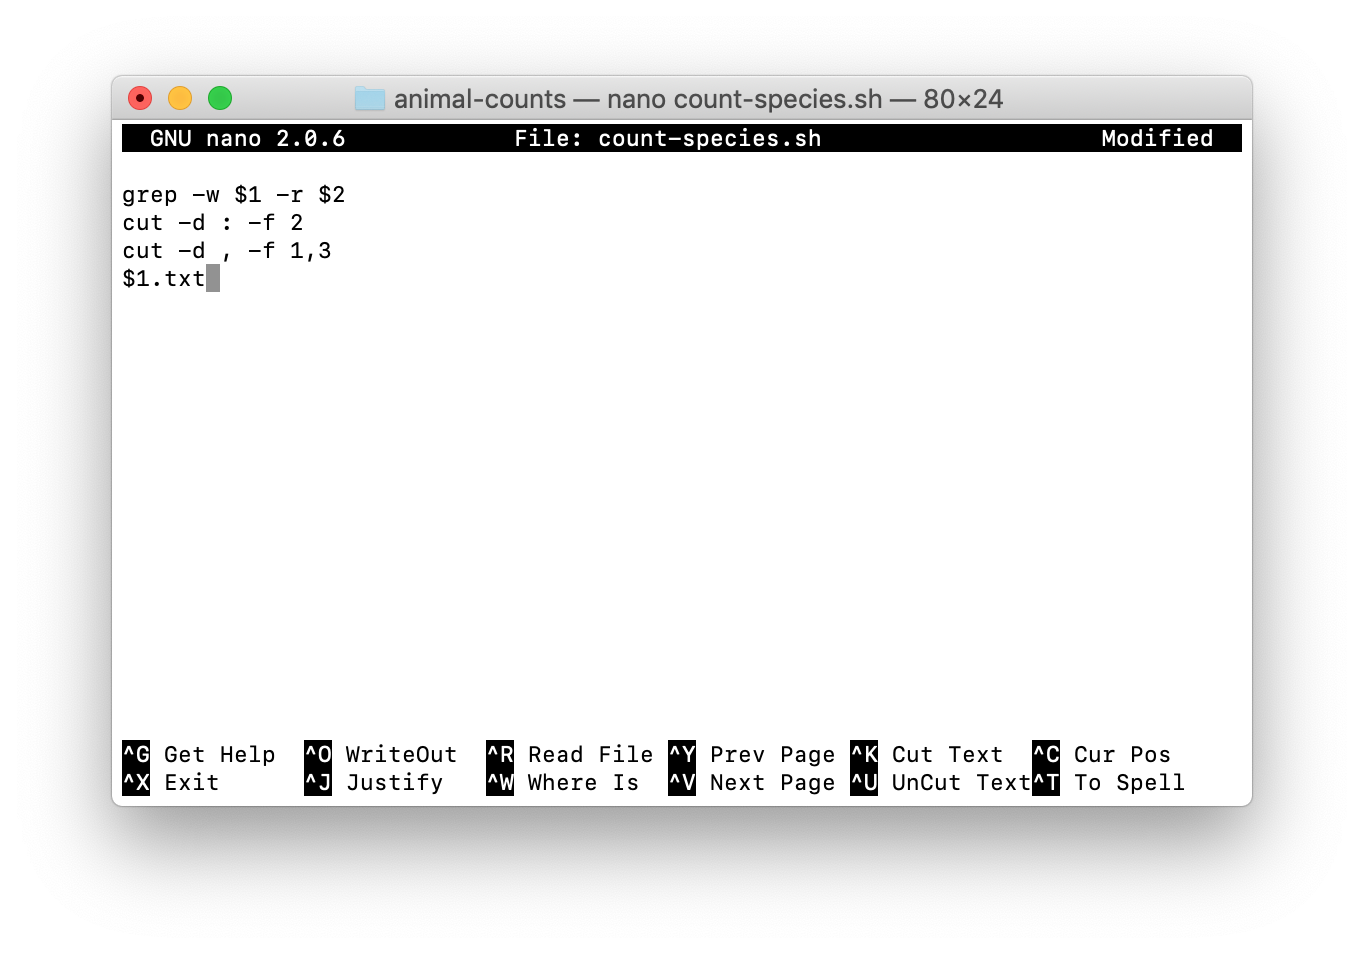
\includegraphics[width=\textwidth]{ftb.png}

\section*{4/9/19 - 11:00am}

\textit{Little Women}

I did the following.

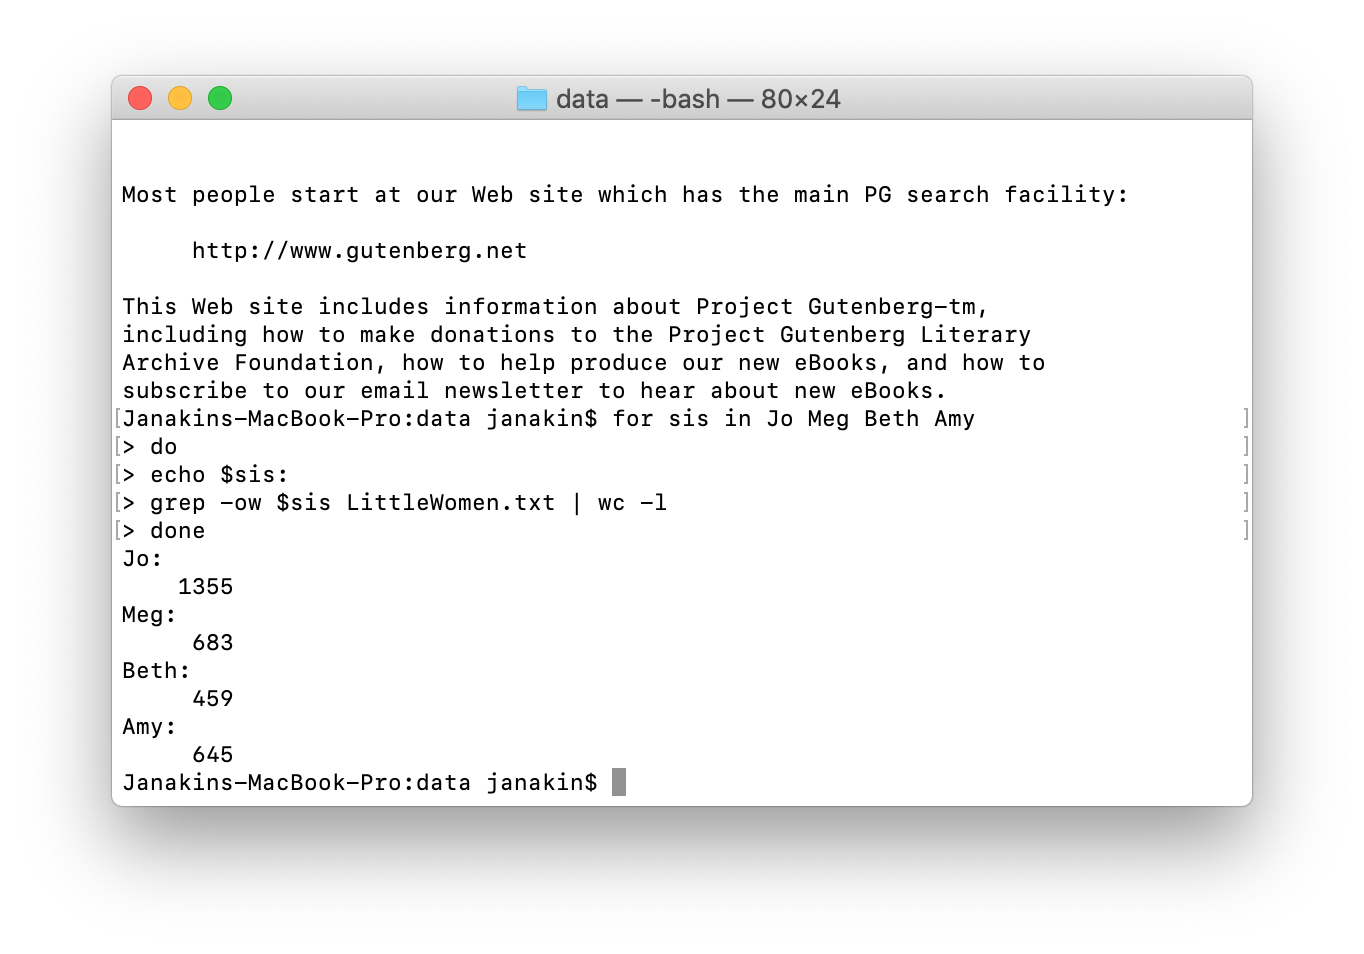
\includegraphics[width=\textwidth]{ftc.png}

\section*{4/9/19 - 11:04am}

Continuing on with the lesson.

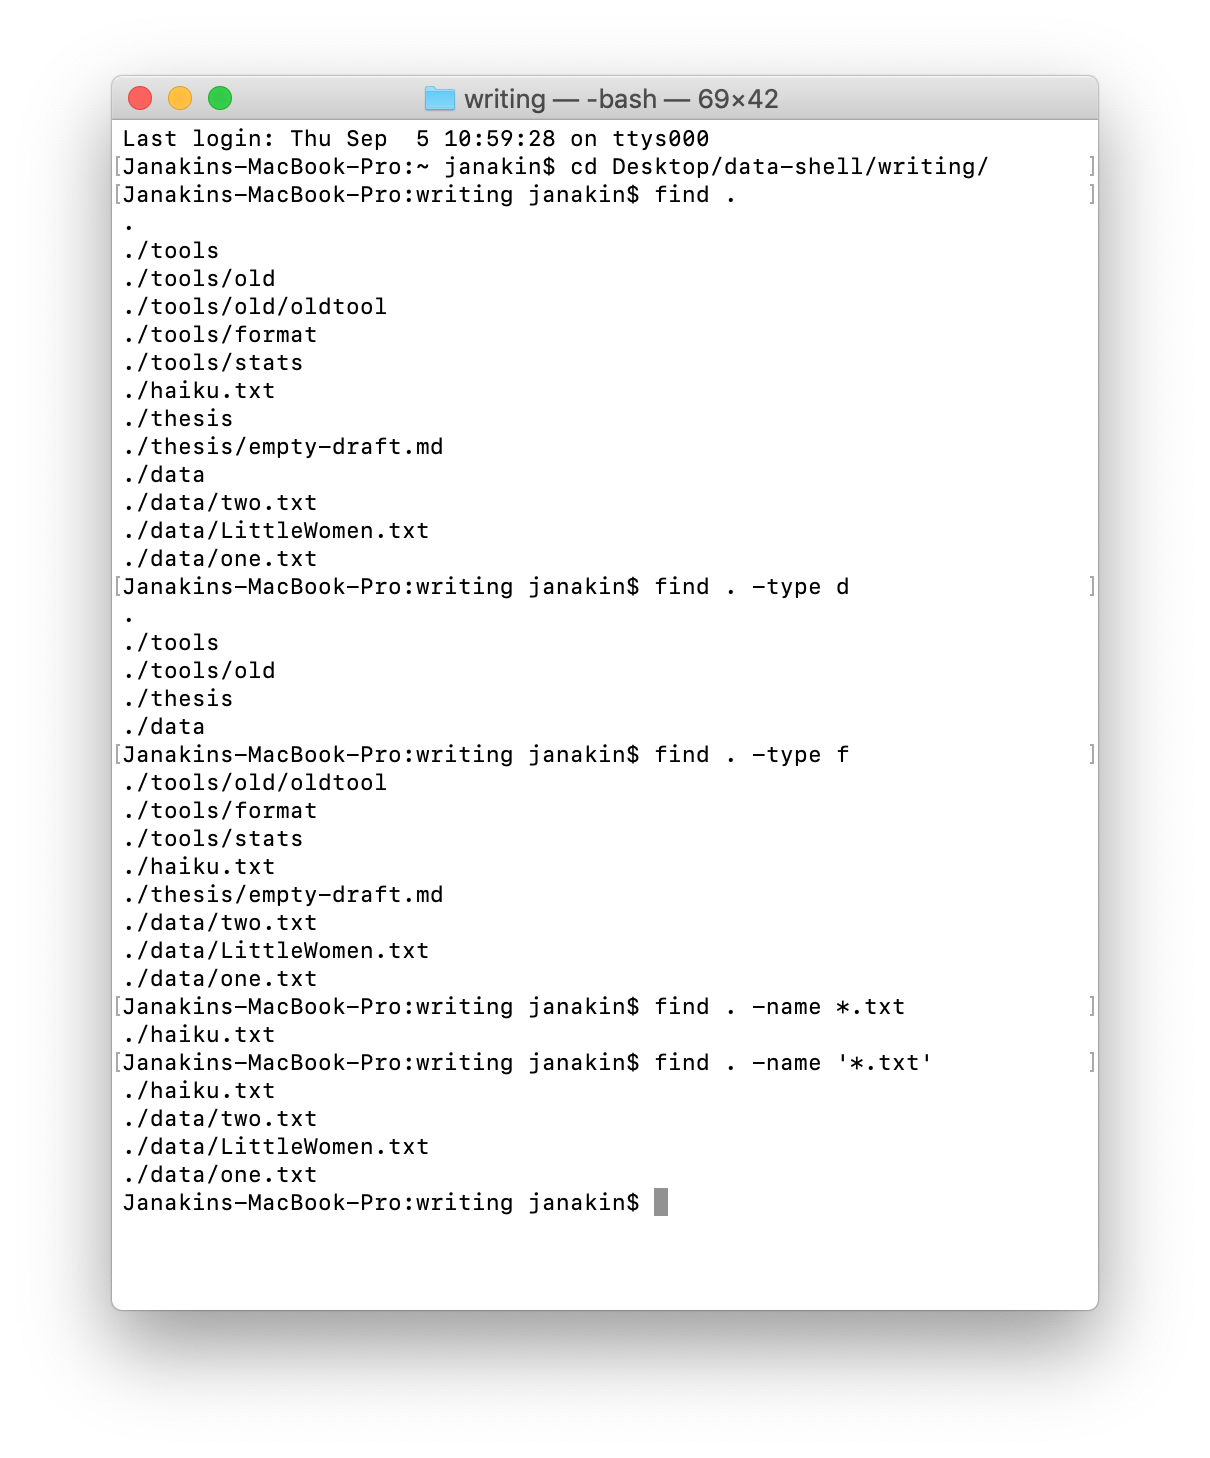
\includegraphics[width=\textwidth]{ftd.png}

\section*{4/9/19 - 11:06am}

\textit{Matching and Subtracting}

The correct answer is 1.

\begin{verbatim}
    find data -name '*s.txt' | grep -v net
\end{verbatim}

\section*{4/9/19 - 11:10am}

\textit{find Pipeline Reading Comprehension}

It will find .dat files, count the number of lines the files have and sort the output numerically.

\section*{4/9/19 - 11:12am}

\textit{Finding Files With Different Properties}

\begin{verbatim}
    find ./ -type f -mtime -1 -user ahmed
\end{verbatim}

\end{document}
